\documentclass[american,titlepage]{ntnuthesis}

\title{An NTNU Thesis \LaTeX{} Document Class}
\shorttitle{An NTNU Thesis Document Class}
\author{Community of Practice in Computer Science Education at NTNU}
\shortauthor{CoPCSE$@$NTNU}
\date{CC-BY \ntnuthesisdate}

\addbibresource{thesis.bib}
\addbibresource{references.bib}

%\input{glossary.tex} % add glossary and acronym lists before document

\begin{document}

\chapter*{Abstract}

In this study, we explored the potential of using Neural Radiance Fields (NeRFs) for novel view synthesis. Our findings show that different NeRF methods perform differently on various scene types in terms of reconstruction quality and computational efficiency. We also found that increasing the number of input images can improve the performance of NeRF methods, but this comes at the cost of longer processing times. Overall, our findings support that NeRFs are effective for novel view synthesis.
\chapter*{Sammendrag}

I denne studien utforsket vi potensialet ved å bruke "Neural Radiance Fields" (NeRFs) for visningssyntese. Våre funn viser at ulike NeRF-metoder fungerer forskjellig på ulike scenetyper når det gjelder rekonstruksjonskvalitet og beregningseffektivitet. Vi fant også ut at å øke antall inndatabilder kan forbedre ytelsen til NeRF-metoder, men dette kommer på bekostning av lengre behandlingstider. Samlet sett støtter funnene våre at NeRF-er er effektive for visningssyntese.

\tableofcontents
\listoffigures
\listoftables
\lstlistoflistings

\printglossary[type=\acronymtype] % Print acronyms
\printglossary                    % Print glossary

\chapter{Introduction}

The advance in Neural Radiance Fields (NeRFs) proposes a new method for reconstructing 3D scenes from 2D images.

By leveraging NeRFs we can create a pipeline that efficiently reconstructs 3D scenes. The reconstructed scenes have many applications, and could be beneficial in applications that require simulated virtual worlds.

This thesis explores how we can leverage NeRFs to reconstruct realistic 3D scenes from 2D images. Further it will explore the limits of NeRFs and see how the capacity can affect how large scenes can be reconstructed.

% and modify an open-source large-scale NeRF pipeline to create a virtual environment of parts of Trondheim.

Research questions:
- 

---



\chapter{Related Work} \label{chap:relatedwork}

% --------------------- Volume rendering ---------------------
\section{Volume rendering} \label{sec:volumerendering} % Most text is directly from sources - rewrite - have now paraphrased it
"Direct volume rendering refers to techniques which produce a projected image directly from the volume data, without intermediate constructs such as contour surface polygons" \cite{max_optical_1995}. It makes it possible to project 2D images from a series of discretely sampled 3D data. A volume renderer may be used to display not just the model's surfaces but also all of its fine details. Many visual effects are volumetric in nature. It is challenging to simulate fluids, clouds, flames, smoke, fog, and dust using geometric primitives. Such effects may be produced more effectively with volumetric models. These models presuppose that a high number of particles in the volume emit, absorb, and scatter light. \cite{ikits_chapter_2007}.

There are multiple ways of rendering a volume. Well-known techniques include ray casting or raymarching, resampling or shear-warp, texture slicing, and splatting. The basic algorithm, visualized in \autoref{fig:volumerendering}, can be broken into four steps:

\begin{itemize}
    \item \textbf{Ray casting:} Cast rays from the image plane into the volume. The volume is often enclosed within a bounding primitive like a cuboid.
    \item \textbf{Sampling:} As the ray enters the volume, sample equally spaced points from the volume. This equidistant sampling builds an intensity profile for the ray, density per volume depth. In the general case where the volume isn't aligned with the ray's direction, the sampling point will be positioned in between voxels, and the values must be interpolated from its adjacent voxels.
    \item \textbf{Shading:} Utilizing the generated intensity profile and a transfer function, we compute the $RGB\alpha$-color and an illumination-value gradient. The gradient vector points in the direction of the greatest increase, indicating where the most rapid increase in illumination is. The samples are colored with their $RGB\alpha$ value and shaded according to the gradient vector and the location of the scene's light source.
    \item \textbf{Compositing:} The final color of the pixel is retrieved by compositing all the shaded samples along the ray.
\end{itemize}

\begin{figure}[h]
    \centering
    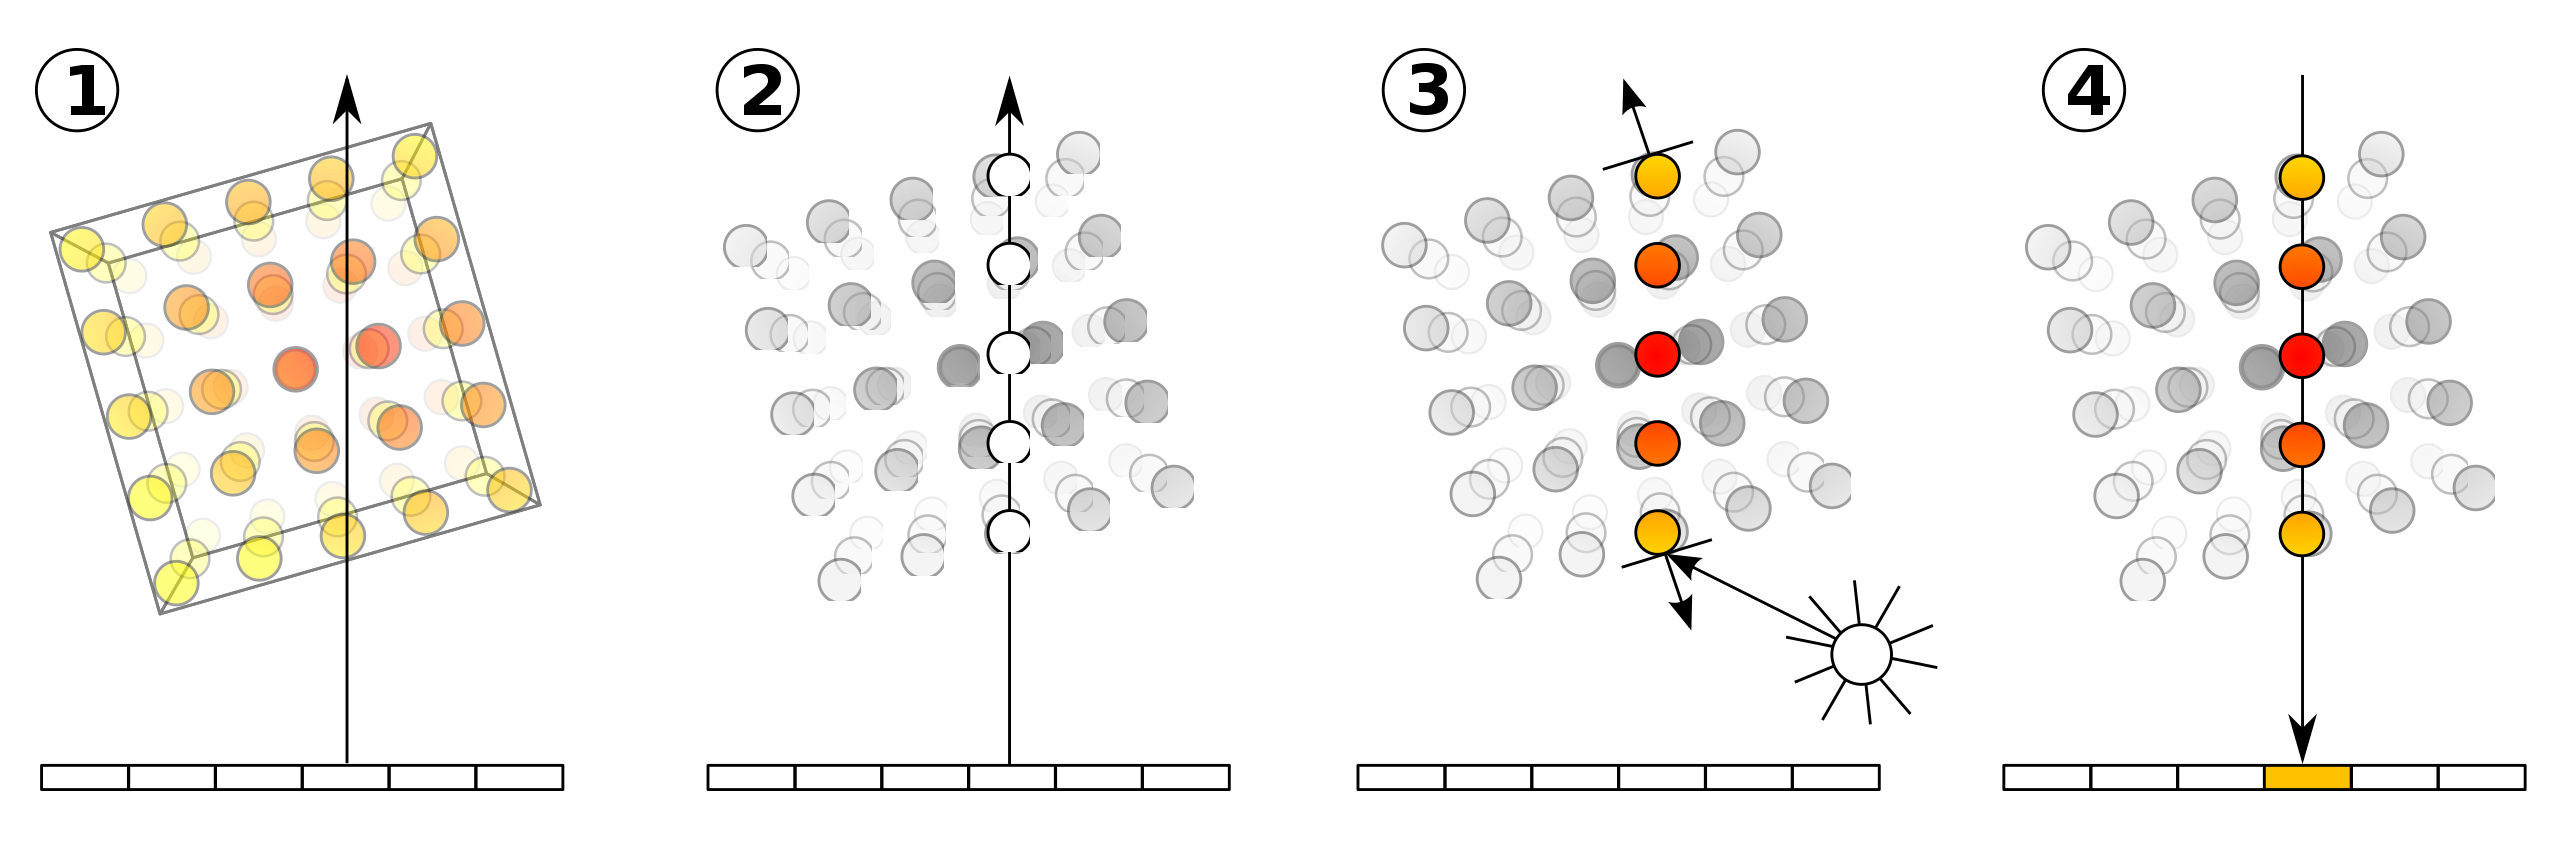
\includegraphics[width=1.0\textwidth]{figures/VolumeRenderingRayCasting.png}
    \caption{The four basic steps of volume rendering \cite{wiki:Volume_ray_casting}. 1) A ray is cast from the image plane into the volume. 2) Points in the volume are sampled. 3) The points are shaded based on their $RGB\alpha$-value and the illumination-value gradients in relationship with the local light source. 4) The final pixel color is composited along the ray.}
    \label{fig:volumerendering}
\end{figure}


After having acquired a 3D data set, rays are cast from the center of the viewing direction (camera origin), through the image plane and into the volume. As the ray enters the volume, an intensity profile is generated. The scalar value per the depth of the volume will be proportional with the density of the volume being traversed.

%Volume rendering enables photorealistic novel view synthesis \cite{xieNeuralFieldsVisual2022}.

\begin{comment}
\subsection{Alpha compositing}
Alpha compositing is the process of combining one image with a background to create the appearance of partial or full transparency \cite{wiki:Alpha_compositing}.

\subsection{Ray marching}
\end{comment}



% --------------------- Neural Fields ---------------------
\section{Neural Fields} % All text is taken from \cite{xie_neural_2022} - rewrite - have now paraphrased it
A field that has been entirely or partially parameterized by a neural network is known as a neural field. The field is a quantity that may be defined for any set of temporal or spatial coordinates. By design, neural fields are both continuous and adaptable. The parameterization of neural fields as MLPs with gradient-defined activation functions is common.\cite{xie_neural_2022}.

A typical neural fields algorithm in visual computing would first, across space-time, sample coordinates and feed them into a neural network to produce field quantities. The field quantities are samples from the desired reconstruction domain of our problem. Then, we apply a forward map to relate the reconstruction to the sensor domain (e.g. RGB image), where supervision is available. Finally, we calculate the reconstruction error or loss that guides the neural network optimization process by comparing the reconstructed signal to the sensor measurement.




% --------------------- Neural Radiance Fields (NeRFs) ---------------------
\section{Neural Radiance Fields (NeRFs)}
Most of the volumetric data we interact with through computer games, movies, and other computer graphic applications, are represented by meshes. A mesh is a collection of vertices, edges, and faces that can be combined in order to define the shape of objects. Meshes are easy to manipulate and interact with. Another common representation of volume is voxels, where a 3D point in space is represented by a value, e.g. a color. Both of these modeling techniques are explicit representations. As we want to increase the resolution of the scene, we have to model increasingly smaller regions of space, i.e. increase the number of voxels/triangle-meshes in the volume. This doesn't scale well as the memory requirements increase as we increase the number of voxels/triangle-meshes. We have to find another way to represent the scene, instead of representing it as explicit blocks in space. NeRF provides an implicit representation of the scene by utilizing a multi-layered perceptron (MLP).

NeRF is a neural volumetric representation. The name, neural radiance fields, gives us a clue as to what it is. It is a field, a space full of particles, where each particle has a given radiance, a color emitted by the particle in a certain direction, and the field is represented with a neural network. NeRF parameterizes 3D scenes as 3D neural fields, mapping 3D coordinates to radiance and density. The 3D scene can subsequently be rendered via volume rendering \autoref{sec:volumerendering}.

% The name, neural radiance fields, gives us a clue as to what it is. It is a field, a space full of particles, where each particle has a given radiance, a color emitted by the particle in a certain direction, and the field is represented with a neural network.

\subsection{Differentiable rendering}
% Change this - directly from the paper
A major breakthrough in 3D reconstruction was the adoption of differentiable rendering (Section 4), which allowed reconstruction of 3D neural fields representing shape and/or appearance given only 2D images, instead of 3D supervision. This has significant implications since 3D data is often expensive to obtain, while 2D images are omni-present. A particularly important social implication is that non-experts can become 3D content creators, without the barrier of specialized hardware. \cite{xieNeuralFieldsVisual2022}



\subsection{NeRF - Representing Scenes as Neural Radiance Fields for View Synthesis}

\begin{figure}
    \centering
    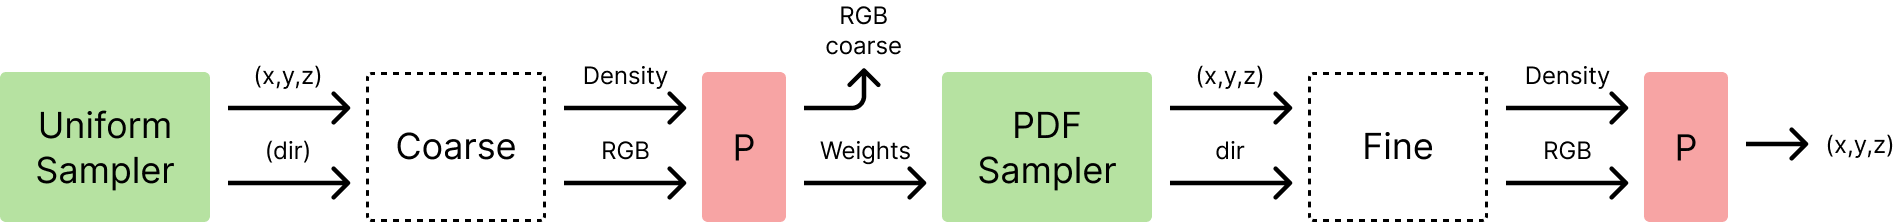
\includegraphics[width=1.0\textwidth]{figures/NeRF_Pipeline.png}
    \caption{Visualization of the NeRF pipeline}
    \label{fig:nerf-pipeline}
\end{figure}

The first paper to present Neural Radiance Fields (NeRFs) was \cite{mildenhall_nerf_2020}. NeRFs provides a method for reconstructing 3D scenes and synthesizing novel views. Given multiple 2D images and their corresponding camera poses, NeRF builds a dataset by sampling points in the volume. The points in the dataset are passed through an MLP in order to predicate the given points' density and color. The predicted density and color values are then composited into a final color which is compared to the reference image pixel's color. The MLP is optimized to minimize the difference between the predicted and reference pixel color.

%NeRF does this by querying an underlying MLP overfit to a specific scene, which represents a continuous volumetric field.
%NeRF renders pixels by emitting rays into the scene. The rays are represented by the ray equation $\pmb{r}(t) = \pmb{o} + t\pmb{d}$ where $\pmb{o}$ is the ray's origin, usually the center of the camera, and $\pmb{d}$ is the ray's direction.

Given multiple 2D images and their corresponding camera poses, which can be approximated with Structure from motion techniques as discussed in \autoref{sec:sfm}, NeRF builds a dataset by sampling points in the volume. Points are sampled along a ray $\pmb{r}(t)$ with origin $o$, the camera's center of projection, and direction $d$. As discussed in \autoref{sec:hierarchicalsampling}, the original paper leverages hierarchical sampling to increase the sampling rate of important parts of the volumetric scene.

%Sample points along a ray $\pmb{r}(t)$, defined by the ray function \autoref{eq:rayfunction}.

\begin{equation}
    \pmb{r}(t) = \pmb{o} + t\pmb{d}
    \label{eq:rayfunction}
\end{equation}

%$\pmb{o}$ is the origin and $\pmb{d}$ is the ray's direction. 

A point $\pmb{x} = \pmb{r}(t_k)$ where $t_k \in t$ is a 3D-coordinate. These 3D coordinates, in conjunction with their viewing direction \textbf{d}, make up the dataset that the MLP is trained on. It's been shown that MLPs have a hard time learning high-frequency signals given low-dimensional input \cite{tancik_fourier_2020}. In order to remedy this, we normalize $xyz$ to lie in the interval of $[-1, 1]$ and increase the signals' dimensionality by applying positional encoding, \autoref{sec:positionalencoding}. The dimensionality of $\pmb{x}$ and its corresponding viewing direction $\pmb{d}$ is increased by applying $\gamma(\cdot)$ \autoref{eq:positionalencoding} to both.

\begin{equation}
    \gamma(p) = [\sin(\pi p), \cos(\pi p), ..., \sin(2^{L-1}\pi p), \cos(2^{L-1}\pi p)]^T
    \label{eq:positionalencoding}
\end{equation}

A predicted color can be retrieved by passing the encoded 3D coordinate and its corresponding encoded camera pose through the MLP $F_{\theta}$. The output of $F_\theta$ is a 4D vector containing a color $RGB$ and a density $\sigma$. In order to retain multiview consistency, NeRF first predicts the volume density $\sigma$ as a function of just the location $\textbf{x}$. Subsequently, the RGB color $\pmb{c}$ is predicted as a function of both the location and viewing direction.


Using $\sigma$ and $\pmb{c}_k$ we can approximate the volume rendering, as discussed in \autoref{sec:volumerendering}, to synthesize a novel view of the scene. The expected color $C(\pmb{r})$ can be derived by \autoref{eq:volumerendering}, which further can be approximated with numerical quadrature as shown in \autoref{eq:numericalquadratureloss}.

%Feed $\gamma(x)$ and its corresponding encoded camera pose given by $\gamma(\theta)$ and $\gamma(\phi)$ into the MLP $F_{\theta}$

\begin{equation}
    C(r) = \int_{t_n}^{t_f}T(t)\sigma(\pmb{r}(t))\pmb{c}(\pmb{r}(t), \pmb{d})dt \quad T(t) = \exp{(-\int_{t_n}^{t_f}\sigma(\pmb{r}(s))ds)}
    \label{eq:volumerendering}
\end{equation}


\begin{align} \label{eq:numericalquadratureloss}
    \hat{C}(\pmb{r}) = \sum_{i=1}T_i \alpha_i \pmb{c}_k, && \text{where}~T_i &= \exp{(-\sum_{j=1}^{i-1} \sigma_j \delta_j)},  \\ 
    && \alpha_i &= (1-e^{-\sigma_i}), \\ 
    && \delta_i &= t_{i+1} - t_i
\end{align}


The transmittance $T(t)$ can be viewed as the probability that the ray doesn't "hit anything", i.e. if the ray continues up until point $t$ or not. $\sigma(\pmb{r}(t))$ and $c(\pmb{r}(t), \pmb{d})$ is the density and color of point $\pmb{r}(t)$, respectively.

Since volume rendering is differentiable, we optimize the loss between the synthesized and ground truth observed image. This is done by calculating the total squared error between the ground truth pixel colors and the synthesized pixel color over all the rays $\pmb{r} \in \mathcal{R}$. Both the coarse and fine networks, as described in \autoref{sec:hierarchicalsampling}, are optimized over.

\begin{equation}
    L = \sum_{\pmb{r} \in \mathcal{R}} \left[\left\| \hat{C}_c(\pmb{r}) - C(\pmb{r}) \right\|^2_2 + \left\| \hat{C}_f(\pmb{r}) - C(\pmb{r}) \right\|^2_2\right]
    \label{eq:nerfloss}
\end{equation}

An overview of the NeRF pipeline can be viewed in \autoref{fig:nerf-pipeline}

\subsubsection{Positional Encoding} \label{sec:positionalencoding}
Positional encoding is one of the many proposed encoding schemes, first introduced in the original NeRF paper. It is a method used to increase the dimensionality of an input vector. It is not to be confused with positional encoding in transformers. It is shown that deep networks are biased toward learning lower-frequency functions. 

\subsubsection{Hierarchical sampling} \label{sec:hierarchicalsampling}
When training a NeRF, different sampling strategies can be utilized. The sampling strategy is an important choice as it is core to how the dataset for the MLP is constructed. In the original NeRF paper they used a sampling strategy called hierarchical sampling. The key notion is that they trained two MLPs, one \textit{coarse} and one \textit{fine}. The coarse MLP uses stratified sampling, as described in \autoref{sec:stratifiedsampling}, where points along the ray are sampled in uniform intervals within each bin. When being trained, the coarse MLP creates a probability distribution function (PDF) of which samples contributed highly to the final predicted RGB value. This PDF is then passed to the fine MLP which sample points along the ray in accordance with the PDF. This strategy of having a coarse network predict the important areas to sample, i.e. the areas that contain a volume, helps the fine network predict a better result. \cite{mildenhall_nerf_2020}

% Point from Mip-NeRF 360. Doesn't fit very well here, but it's a good point!
The only reason why the coarse network is supervised is to guide the sampling of the fine network. This is the motivation behind improvements in e.g. Mip-NeRF 360

\subsubsection{Stratified sampling} \label{sec:stratifiedsampling}
Stratified sampling is a sampling method. It has proven benefits in machine learning as it helps prevent overfitting. The sampling method consists of two steps:

\begin{itemize}
    \item \textbf{Partition the dataset into strata:} In the case of NeRF, a strata is the points contained within a bin $\pmb{x} \in [t_i, t_i+1]$ along the ray $\pmb{r}(t)$. The population/size of a strata can vary based on predefined functions. Importance sampling can be achieved by increasing the size of the strata in accordance with a PDF.
    \item \textbf{For each stratum, apply simple random sampling:} 
\end{itemize}

\begin{figure}[h]
    \centering
    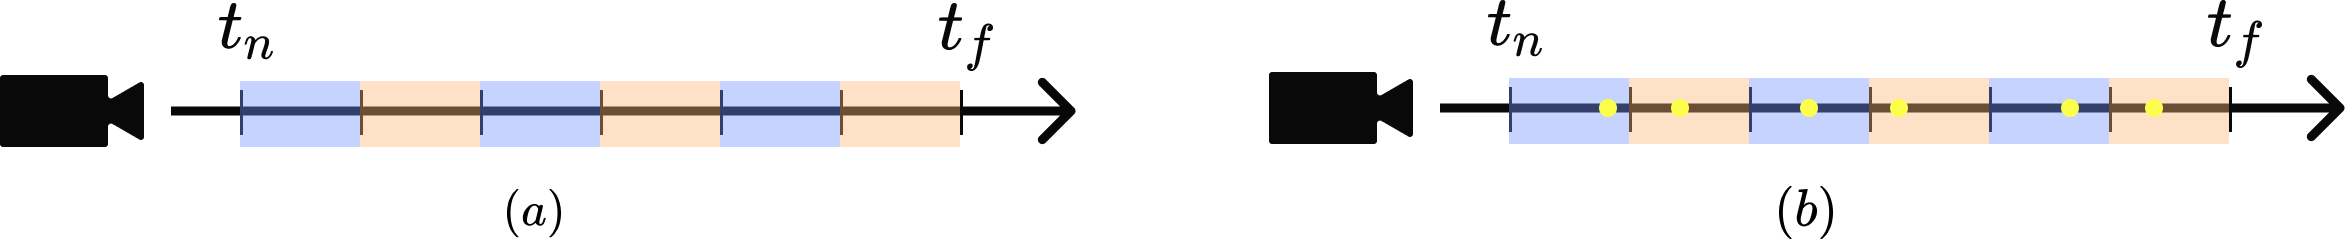
\includegraphics[width=1.0\textwidth]{figures/StratifiedSampling.png}
    \caption{a) The ray is uniformly binned from the near bound $t_n$ to the far bound $t_f$, defining the strata. b) random points are sampled from the bins.}
    \label{fig:stratifiedsampling}
\end{figure}

\subsection{Block NeRF}
Block NeRF is a paper 

\subsection{Appearence embeddings}

\subsection{Learned pose refinement}

\subsection{Visibility map}





% --------------------- Other models that Nerfacto builds on ---------------------
\section{MIP-Nerf}\label{sec:mipnerf}
% REWRITE
NeRF shows good performance when all training and testing photos are taken at about the same distance from the scene, and it doesn't have to reason about scale or aliasing. When you add more cameras, pulled away from the scene, NeRF starts to break down, because it's a single-scale model now trying to solve a multi-scale problem. Renderings from the NeRF will show aliasing artifacts in distant views and excessive blur in close-up views.

A solution to this problem would be to adapt a solution that is used in offline ray tracing, supersampling. With supersampling, we would march multiple rays through the same pixel's footprint. This technique doesn't solve the issue of aliasing effects, but the rendered image would look better. However, doing so would be very computationally expensive and it would increase the already very long training times of NeRF, which already depends on querying an underlying MLP hundreds of times for a single ray.

Another sampling strategy apart from casting rays through each pixels' footprint would be to cast a cone, as seen in \autoref{fig:mipnerffrustums}. The cone's radius is determined by the size of the pixel's footprint on the image plane, so that the cone models the whole volume of space visible by the pixel. When the pixel's cone is rendered, all the content within that visible volume will be averaged out, instead of rendering out whatever intersects with the infinitely narrow ray that was cast by NeRF. The cone is divided into conical frustums. The frustums are approximated with a multivariate Gaussian since they're easier to manipulate and have a closed-form solution.

\begin{figure}[h]
    \centering
    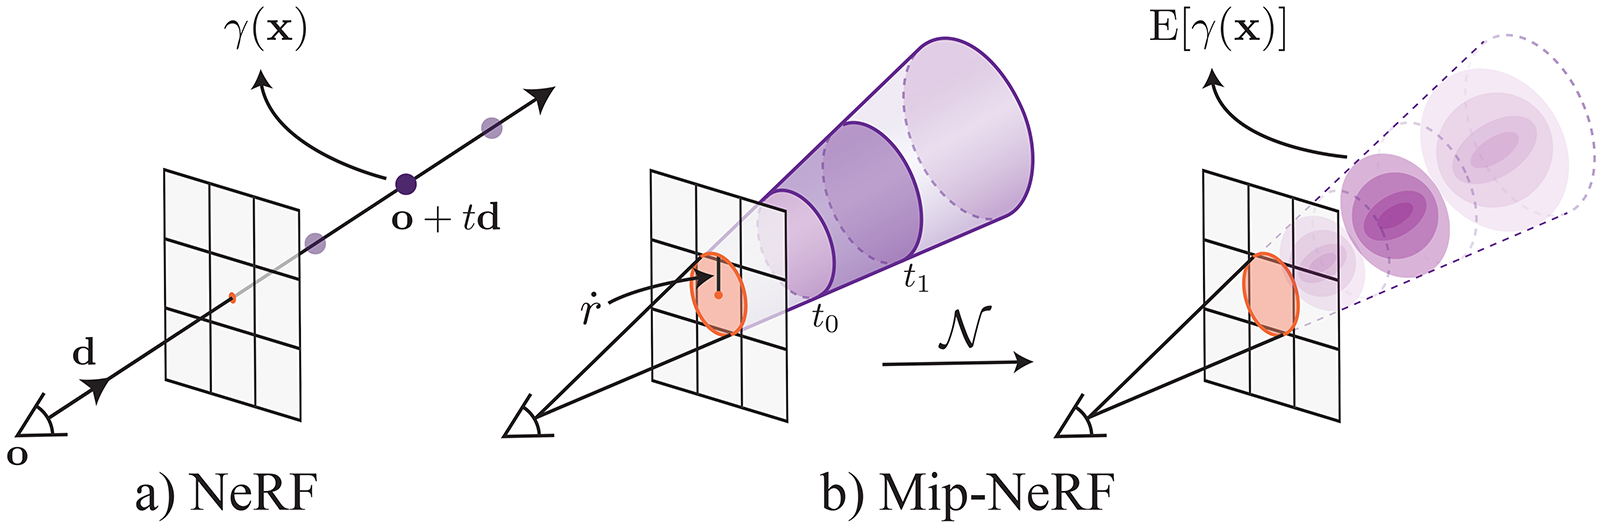
\includegraphics[width=1.0\textwidth]{figures/MipNeRFFrustums.png}
    \caption{Cones are cast through the pixels' footprint and into the volume.}
    \label{fig:mipnerffrustums}
    \cite{figure:mipnerffrustum}
    \label{fig:my_label}
\end{figure}


Instead of positionally encoding a single point along the ray, we compute the expected positional encoding with respect to the Gaussian that we've constructed. With this encoding, mip-NeRF is able to reason about the scale of its input by looking at the scale of the encodings. This lets the model understand the difference between small and large volumes. This encoding scheme is called integrated positional encoding (IPE), and has a simple closed-form that can be computed quickly.

Inspiration to this method is taken from mipmapping which traditionally has been used to prevent aliasing in computer graphics pipelines. A mipmap is a pre-filtered set of discretely downsampled signals, very often images, which helps speed up rendering as the responsibility of anti-aliasing is shifted to a precomputation phase. Mip-NeRF extends NeRF to simultaneously represent the pre-filtered radiance field for a continuous space of scales, thereof "mip-NeRF".





\section{Mip-NeRF 360} \label{sec:mipnerf360}
Focuses on unbounded scenes: Scenes with main object of interest in front of an elaborate background. It addresses challenges with extending mip-NeRF to unbounded scenes. There are primarily three techniques proposed by MIP-NeRF 360 which we'll cover in this section.

\textbf{Representation}:
The first challenge with extending mip-NeRF to unbounded scenes is that unbounded scenes are large, but mip-NeRF requires a bounded domain.

Problem: Unbounded scenes are large, but mip-NeF needs a bounded domain
Solution: Apply a Kalman-like warp to mip-NeRF Gaussians to warp the mip-NeRF into non-Euclidean space.

All the Gaussians outside a ball of radius one will smoothly be warped into a non-euclidean space within a radius two ball. This non-Euclidean space is used to represent the input to the MLP. 

\textbf{Efficiency}
Problem: Large scenes require more network capacity, but using a large MLP is too expensive (given that you have to query it hundred of times for a single ray)
Solution: "Distill" scene geometry from a large NeRF MLP into a small MLP while training
Train a small proposal MLP to bound the geometry predicted by a large NeRF MLP which makes training ~3 times faster

Feed a set of points through a proposal MLP which produces a set of weights, but no colors. Those weights are used to resample the ray, the same way the weights from the coarse network in the original NeRF paper is used as a PDF to guide sampling. The resampled points are then used to render a color, which is supervised. 

Instead of supervising the proposal MLP to accurately reconstruct the image, we supervise its output weights to be consistent with the output weights from the NeRF MLP, i.e. calculate the loss between the output weights from the NeRF MLP and the proposal MLP. Because of this we can have a very small proposal MLP which we query very frequently, and a larger NeRF MLP which is queried relatively few times.

To make this work we need a loss function that encourages histograms with different bin endpoints to be consistent with one another. To achieve this we make some strong assertions on the relation between the two distributions, summarizing the same underlying, true distribution. The loss function will penalize any excess mass that violates the upper bound imposed on the proposal MLP.

\textbf{Ambiguity}
Problem: 3D reconstruction becomes more ambigious as you increase the scene size. Results in more artifacts
Solution: Utilize a novel regularizer designed specifically for mip-NeRF ray intervals.

The regularizer encourages each rays' histogram to be as close to a delta function as possible. 


\section{Nerfacto}
Nerfacto builds on the ideas from mip-NeRF 360


% --------------------- removing the requirement of known or pre-computed camera parameters ---------------------
\section{Removing requirement of known camera parameters}
BARF, NeRF--, Block-NeRF


% --------------------- Structure from motion ---------------------
\section{Structure from motion} \label{sec:sfm}
Structure from motion is a technique for estimating 3D structures from sequences of 2D input images. In NeRF it is used a preprocessing tool for retrieving camera poses of the input images. In most NeRF methods, accurate camera poses are a strict requirement, although some papers have experimented with removing the need for pose supervision \cite{lin_barf_2021}.

\subsection{COLMAP} \label{sec:colmap}
COLMAP is a general-purpose Structure-from-Motion (SfM) \cite{schoenberger2016sfm} and Multi-View Stereo (MVS) \cite{schoenberger2016mvs} pipeline. The general overview of the pipeline contains the following steps:
\begin{itemize}
    \item Feature detection and extraction
    \item Feature matching and geometric verification
    \item Structure and motion reconstruction
\end{itemize}

During the first step, SIFT-features \cite{Lowe2004} are extracted. Sparse feature points in the image are found and their appearences are described using numerical descriptors.

% TODO: Elaborate on the different match-options; Exhaustive Matching, Sequential Matching, Vocabulary Tree Matching. Runtimes, found in the paper, can be added to appendix.

\begin{comment}
Exhaustive matching:
time complexity: O(n^2), where n is the number of images
memory complexity: O(n) for storing all images, O(n^2) for storing the results of the matching process

Sequential matching:
time complexity: O(n * k), where n is the number of images and k is the number of adjacent images each image is matched against
memory complexity: O(n * k)

Vocabulary tree-based matching:
time complexity: O(n^2), assuming that the size of the vocabulary tree is constant and not a function of the number n of images
memory complexity: O(n * k), where k is the number of top-retrieved images that each image is matched against
There is definitively literature on the topic of the time and memory complexity of vocabulary tree-based matching and image retrieval
\end{comment}

During the second step, features are matched. Correspondences between the feature points are matched across different images, leveraging feature matching and geometric verification. There are different options for matching algorithms. Exhaustive matching would match every image against every other image, leading to the best reconstruction results. The time complexity is not an issue if the number of images are relatively low (several hundreds). Another option is sequential matching which is useful if the captured images are in sequential order, e.g. if they're sampled from a video.

During the third step, structure and motion is reconstructed. First COLMAP will generate a sparse reconstruction of the scene, extracting the camera poses. The sparse output serves as input to the Multi-View Stereo to recover a dense representation of the scene. The dense representation estimates the dense surfaces. As COLMAP is used as a preprocessing step for retrieving the camera poses of input images, the pipeline is usually ceased after the sparse reconstruction.

\begin{table}[h] \label{tab:colmap-complexity}
\begin{tabular}{lcc}
\hline
Matching algorithm & \multicolumn{1}{l}{Time complexity} & \multicolumn{1}{l}{Space complexity} \\ \hline
Exhaustive         & $\mathcal{O}(n^2)$       & $\mathcal{O}(n^2)$  \\
Sequential         & $\mathcal{O}(n k)$ & $\mathcal{O}(n k)$        \\
Vocabulary Tree    & $\mathcal{O}(n^2)$*       & $\mathcal{O}(n k)$  \\ \hline
\end{tabular}
\caption{An overview of the time and memory complexities of a selection of COLMAP matching algorithms. For sequential matching $k$ is the number of adjacent images each image $n$ is matched against. For Vocabulary tree-based matching, $k$ is the number of top-retrieved images that each image $n$ is matched against.}
\end{table}




% --------------------- Evaluating NeRFs ---------------------
\section{Evaluating NeRFs}
Evaluating the quality of NeRFs is inherently hard since it's a visual modality. After a NeRF is trained it will eventually be used to render an image. Image similarity metrics are consequently the most important metric to evaluate the quality of a NeRF. The assessment of image similarity has been a long-standing challenge in computer graphics, but the following metrics are commonly used throughout most papers comparing NeRFs.

\subsection{PSNR - Peak Signal-to-Noise Ratio}
PSNR is a common measure for quantifying reconstruction quality for images and videos. It builds upon MSE which measures the absolute difference between each pixel in two images $I_1$ and $I_2$.

\begin{align} 
    \text{PSNR} &= 20 \cdot \log_{10}\left(\dfrac{MAX_I}{\sqrt{\text{MSE}}}\right) \label{eq:psnr}, \ \text{where} \\ 
    %\\ &= 20 \cdot log_{10} (MAX_I) - 10 \cdot log_{10}(MSE)
    \text{MSE} &= \dfrac{1}{m n} \sum_{i = 0}^{m-1} \sum_{j = 0}^{n-1} \left[I_1(i,j) - I_2(i, j) \right]^2, \ \text{and} \label{eq:mse}
\end{align}

$MAX_I$ represents the dynamic range of an image, i.e. the highest pixel value that the picture may contain. This is 255 when pixels are represented with 8 bits per sample. In more general terms, $MAX_I$ is $2^B-1$ when samples are recorded with $B$ bits per sample. Due to the high dynamic range of many signals, PSNR is typically expressed as a logarithmic number using the decibel (dB) scale.

\subsection{SSIM - Structural Similarity}
Although MSE and PSNR are good measures of the reconstruction error, they don't examine an image the same way humans do. We don't compare pixel-value to pixel-value in order to conclude if two images are similar, we look at it in a more holistic way. SSIM tries to capture this by instead comparing luminance $l$, contrast $c$ and structure $s$ between two windows $x$ and $y$ of common size $N \times N$.

\begin{align} \label{eq:ssim}
    \text{SSIM}(x, y) &= l(x,y)^\alpha \cdot c(x,y)^\beta \cdot s(x,y)^\gamma \qquad \text{with } \alpha, \beta, \gamma = 1 \\
    &= \dfrac{(2\mu_x \mu_y + c_1)(2\sigma_{xy} + c_2)}{(\mu_x^2 + \mu_y^2 + c_1)(\sigma_x^2 + \sigma_y^2 + c_2)}
\end{align}

\begin{comment}
\begin{itemize}
    \item $\mu$ represents the pixel sample mean for both $x$ and $y$,
    \item $\sigma^2$ represents the variance for both $x$ and $y$,
    \item $\sigma_{xy}$ represents the covariance of x and y,
    \item $c_1 = (k_1L)^2$, $c_2 = (k_2L)^2$ are variables to stabilize the division with weak denominator,
    \item $L$ represents the dynamic range of the pixel-values,
    \item $k_1 = 0.01$, $k_2 = 0.03$ by default   
\end{itemize}
\end{comment}

SSIM is bounded by $-1 \leq \text{SSIM} \leq 1$ where $1$ implies perfect correlation, $0$ implies no similarity, and $-1$ implies perfect anti-correlation.

\subsection{LPIPS - Learned Perceptual Image Patch Similarity \cite{zhang_unreasonable_2018}}
LPIPS is a perceptual similarity metric based on deep network activations. Where MSE, PSNR and SSIM uses relatively shallow functions in order to determine similarity across images, LPIPS leverage deep neural networks to obtain a metric that perceives similarity the same way humans do. Image patches with a low LPIPS score are perceptually similar.

\begin{figure} [h]
    \label{fig:lpips}
    \centering
    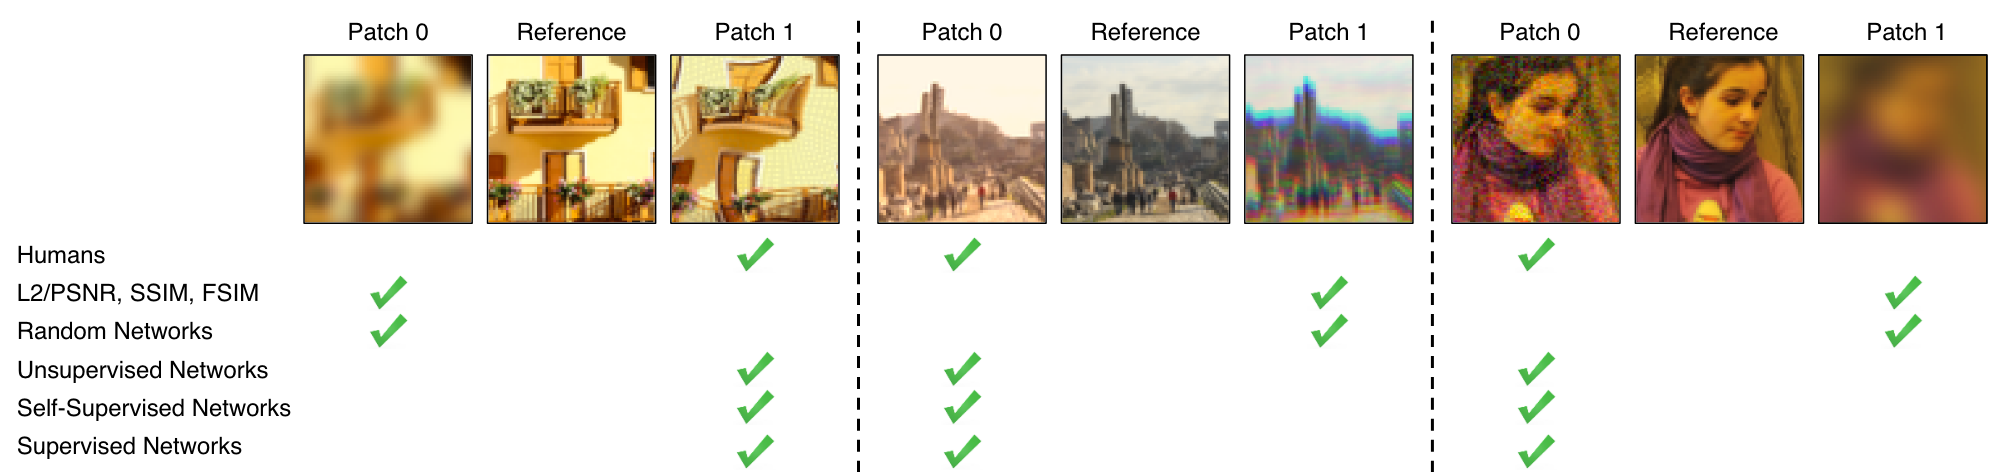
\includegraphics[width=1.0\textwidth]{figures/LPIPS.png}
    \caption{LPIPS is trained to perceive image similarity the same way humans do. The dataset used to train the similarity metric contains two types of perceptual judgements, Two Alternative Forced Choice (\pmb{2AFC}) and Just Noticeable Differences (\pmb{JND}). With 2AFC people were asked to select which of the distorted images was "closer" to the reference. With JND people were presented with 2 image patches, one reference and one distorted, and asked if they were the same.}
    \label{fig:my_label}
\end{figure}

%The metric determines how similar two image patches' activations are, for a given network. It's been demonstrated that this metric closely matches human perception. Image patches with a low LPIPS score are perceptually similar.


\chapter{Method}

The method chapter of this paper describes the process of generating Neural Radiance Fields (NeRFs) using software to test multiple different methods. NeRFs are a novel approach to computer graphics that have shown promising results in recent studies. In this chapter, we will cover the five key steps involved in the NeRF generation process: capture, process, training, rendering, and evaluating. Lastly we'll have a look at the dataset captured and used throughout the experiments.

Our approach to generating NeRFs leverages state-of-the-art software that allows us to test and compare multiple different methods. We have selected a range of methods to evaluate, including both traditional and cutting-edge techniques. This will provide valuable insights into the strengths and limitations of different approaches to NeRF generation.

In the capture step, we will describe the process of acquiring the necessary data to train the NeRF model. This includes details of the equipment and techniques used to capture high-quality images of real-world scenes.

The process step involves preprocessing the captured data to prepare it for use in training the NeRF model. This includes tasks such as downscaling, feature extraction, and global adjustment of the input data. We will describe the specific methods and algorithms used for these tasks.

The training step is where the NeRF model is actually learned from the processed data. %We will describe the specific neural network architecture and training algorithms used, as well as the hyperparameters that were applied. %We will also discuss any challenges or obstacles that we encountered during training, and how we addressed them.

In the rendering step, we will describe how the trained NeRF model is used to generate novel images of the scene. This includes details of the rendering algorithms and techniques used.%, as well as any post-processing steps that were applied.

Finally, in the evaluating step, we will describe how we quantitatively and qualitatively assessed the quality of the generated NeRFs. %This will include a discussion of the metrics and benchmarks used, as well as a comparison of the results to previous work in the field.

Overall, this method chapter provides a comprehensive description of the process of generating NeRFs, from data capture to evaluation.

\begin{comment}
Describe the pipeline used to generate NeRFs

- Capture (video, image, polycam, etc.)
- Process (COLMAP, or direct extraction from e.g. Polycam)
    - Configuration of COLMAP
- Train (Different models)
    - Configuration of model
- Render (Real-time rendering vs. slow rendering)
- Evaluate (PSNR, SSIM, LPIPS)
- Export

- Pipelines created
    - Pipeline to test 
\end{comment}

\section{Nerfstudio}
With the magnitude of different published methods regarding NeRF, some with corresponding source code and some not, it's not trivial to compare them on self-captured data. In the experiments, I have leveraged an open-source project named Nerfstudio. It is an API that streamlines the creation, training, and visualization of NeRFs. The components that make up NeRFs are modularized in a way that allows interpretable implementation of different NeRF methods. In addition, it ships with implemented versions of some of the most important published methods to date for real-world captures; NeRF, mip-NeRF, and instant-NGP.

\section{Nerfacto}
\begin{figure}[!h]
    \centering
    %\hspace*{-48px}
    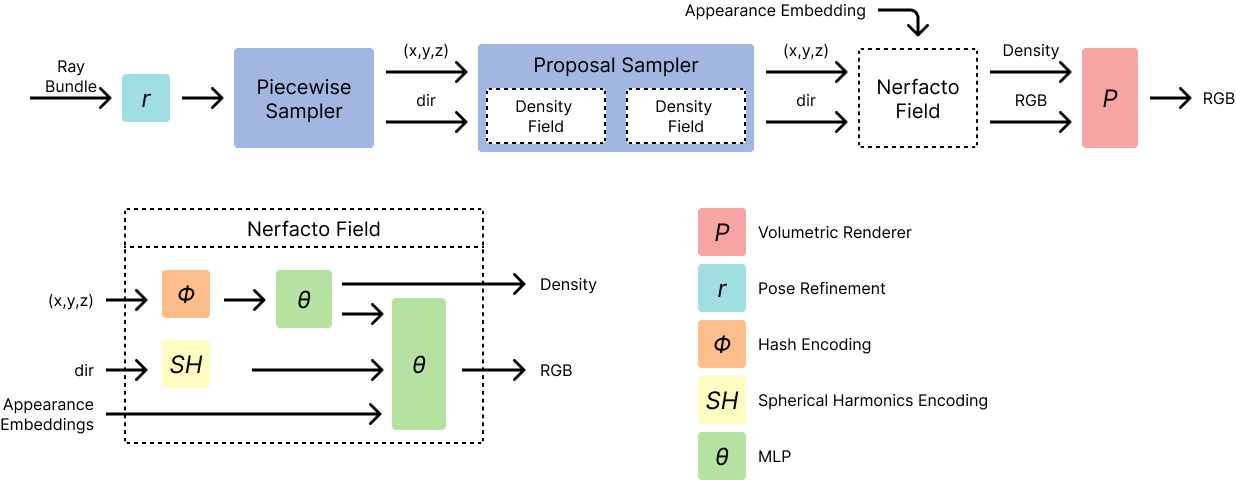
\includegraphics[width=1.0\textwidth]{figures/nerfacto-pipeline-overview.png}
    \caption{}
    \label{fig:nerfacto-pipeline-overview}
\end{figure}
Nerfstudio also provides its own method dubbed "Nerfacto". The method isn't published work, but leverages techniques from several other published methods which have proved to work well for real data captures. The techniques used in Nerfacto result in a method that strikes a great balance between quality and speed. Most of the techniques highlighted by Nerfacto have already been discussed in \autoref{chap:relatedwork}, but I'll recap and elaborate on a few here.

\textbf{Camera pose refinement}, as described in \autoref{sec:camera-pose-refinement} is a technique proposed to reduce the impact of imperfect camera poses. It's a very effective measure to reduce cloudy artifacts and increase the sharpness and overall quality of the resulting 3D representation.

\textbf{Per image appearance conditioning}, as described in \autoref{sec:appearance-embeddings}, is a technique that allows the NeRF to process and represent 3D scenes with variable lighting, exposures, weather, and post-processing effects. In Nerfacto, the appearance embedding is a vector of size 32, which is concatenated with the viewing direction before it's passed through the MLP.

\textbf{Hash encodings} were proposed in \cite{muller_instant_2022}. This parametric encoding differs in how spatial data is represented. In the original NeRF paper, the location \textbf{x} is represented by a positional encoding. With the multiresolution hash encoding, the location \textbf{x} is represented in a hash table by a linear interpolation of its closest vertices at multiple resolutions. This parametric encoding has several advantages in terms of computational effectiveness, resulting in several magnitudes of increased training and inference speed. Although you impose a larger memory cost by allocating several hash tables, the number of required parameter-updates per backpropagation is severely reduced. In Nerfacto, 16 hash tables with $2^{19}$ rows, each storing a feature vector of size 2, are allocated. The subsequent MLP has a very low capacity, with only one hidden layer containing 64 neurons. An overview of the multiresolution hash encoding can be seen in \autoref{fig:instant-ngp-hash-encoding}.

%The only difference is essentially how spatial data is represented, i.e. parametric encoding. Instant-NGP encodes spatial data at multiple resolutions using hash tables, thereof the name multiresolution hash tables. During backpropagation, the MLP's weights and the feature vectors in the hash tables are both updated.
%In a fully connected MLP, every weight and bias must be updated on back-propagation. With parametric encodings, only a very small number of feature vectors must be updated. Also, by reducing the size of the MLP, such parametric models can be trained to convergence much faster without sacrificing approximation quality. You trade a larger memory footprint by allocating hash tables, but in return you have to update a far lower number of trainable parameters per back-propagation, leading to an increased training and inference speed.

\begin{figure}[h]
    \centering
    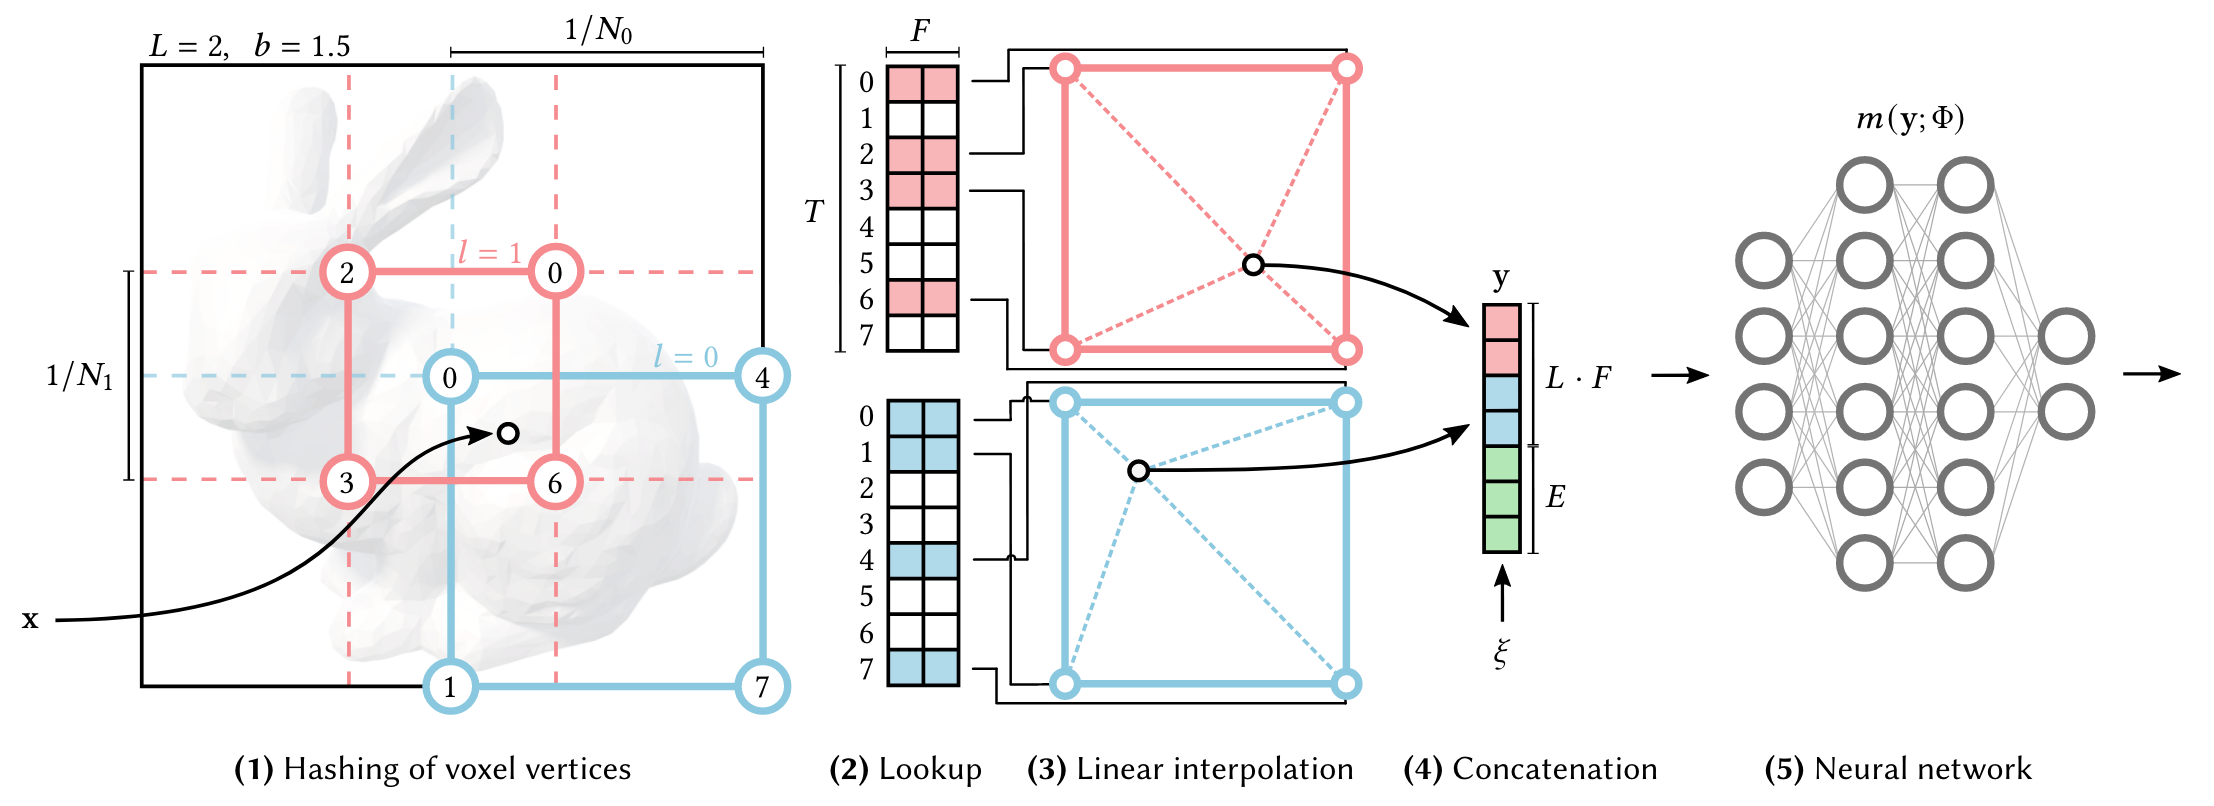
\includegraphics[width=1.0\textwidth]{figures/instant-ngp-hash-encoding.png}
    \caption{Illustration of the multiresolution hash encoding in 2D, Figure 3 \cite{muller_instant_2022}.}
    \label{fig:instant-ngp-hash-encoding}
\end{figure}

\textbf{Proposal sampling} is a sampling technique discussed in \autoref{sec:mipnerf360}. Nerfacto extends the proposal sampler used in mip-NeRF 360 by utilizing two density functions implemented as small fused-MLP with hash encodings \cite{muller_instant_2022}. This provides accurate and fast density estimations.

\textbf{Scene contraction}, as described in \autoref{sec:mipnerf360}, is a technique proposed in \cite{barronMipNeRF360Unbounded2022} to extend mip-NeRF to support unbounded scenes.

\section{Capture}
%- Video, image, polycam, etc. ✅
The different datasets have primarily been captured with an iPhone 13 Pro Max. The iPhone features three lenses that enable captures ranging from ultra-wide to telephoto. Using the ultra-wide option has proved helpful in the pipelines where COLMAP has to be leveraged as it captures more of the scene and more easily enables overlap between the frames. The resulting NeRF-renderings haven't seemed distorted. When capturing video or images for a NeRF it's important that the scene is well-lit, that you capture non-blurry images, and that there are no transient objects present.

Polycam is a "LiDAR \& 3D Scanner for iPhone \& Android". It has multiple settings for performing photogrammetry and LiDAR scans, but most importantly it enables export of images with corresponding camera poses. This is very useful as Nerfstudio has created an integration that reads the camera poses generated by Polycam and transforms it into Nerfstudio's data format. This enables skipping COLMAP entirely from the pipeline. Polycam doesn't support wide camera options, resulting in the need to manually record more of the scene.
%The quality of the camera poses are relatively good.

\section{Process}
%- COLMAP, or direct extraction from e.g. Polycam 
%- Configuration of COLMAP
The data processing step for constructing a NeRF are usually the same across different models. It's a step for creating the dataset of images with corresponding camera poses and is comprised of creating a set of images from a video, scaling the images to a preferred size, and lastly utilizing an algorithm to extract the corresponding camera poses. If you a priori have access to the input images and refined camera poses, as is the case with the Polycam-integration, there's not much pre-processing necessary. All the experiments in this paper leverage Nerfstudio which has its own data processing pipeline API that includes support for video, images, and Polycam-data. For video input, FFMPEG\cite{tomar2006converting} is first used to grab image frames from the video at specified densities, by default ~300 frames. When a set of images is acquired, the images are scaled down in fractions of the original image size. The scaling of the images is done as it's been obeserved that training on images larger than 1600px along the longest dimension has diminishing returns. COLMAP is then used for extracting the camera poses from the set of input images. The choice of matching algorithm, as discussed in \autoref{sec:sfm}, is primarily the only setting you have to tweak for COLMAP.

\begin{lstlisting}[
    caption={Example of running Nerfstudio's process-script. Reference the \href{https://docs.nerf.studio/en/latest/index.html}{documentation} for details.},
    label=code:process,
    language=bash]
$ data_path={nerfstudio/data/your-data-folder}
$ ns-process-data {video, images, polycam} --data $data_path 
  --output-dir $data_path/output
\end{lstlisting}

%COLMAP and FFMPEG \cite{tomar2006converting} are the main data processing tools. FFMPEG is used to grab image frames from the video at specified densities, by default ~300 frames. COLMAP is then used for extracting the camera poses from a set of input images. The choice of matching algorithm, as discussed in \autoref{sec:sfm}, is primarily the only setting you have to tweak for COLMAP.
%Most of the experiments use the default number of frames and the default COLMAP matching algorithm.

\section{Train}
%- Configuration of model
During training, the parameters in the model are trained to represent the 3D scene. For the Nerfacto-model, this entails backpropagating the error and updating both the NeRF MLP and the proposal MLP. For the instant-ngp-model, the small MLP and the feature vectors contained in the multiresolution hash tables are updated.

The training has been conducted with different models, varying amounts of data, and for different scenes. All the configurations have been adjusted with Nerfstudio's API. By default, the dataset is created from ~300 frames and the corresponding camera poses. All the experiments have been trained for 30'000 epochs. The specific parameters for each model is shown in \autoref{app:additional}.

\begin{lstlisting}[
    caption={Example of running Nerfstudio's train-script with the nerfacto model. Reference the \href{https://docs.nerf.studio/en/latest/index.html}{documentation} for details.},
    label=code:train,
    language=bash]
$ data_path={nerfstudio/data/your-data-folder}
$ ns-train nerfacto --data $data_path
\end{lstlisting}

\section{Render}
%- Real-time rendering vs. slow rendering
During rendering, the trained NeRF is queried along a camera path to output a series of images. The camera path contains information about the keyframes to be rendered, the camera-to-world matrices, and data such as render height and width, FPS, and video duration. In Nerfstudio, a camera path can simply be created in their real-time rendered viewer. The camera path can later be exported and used across models trained on the same data to qualitatively compare them.

%The render output can also be tweaked by tuning sampling rates contained in the \textit{config.yml}-file that is generated after you've trained the NeRF.

\begin{lstlisting}[
    caption={Example of running Nerfstudio's render-script. Reference the \href{https://docs.nerf.studio/en/latest/index.html}{documentation} for details.},
    label=code:train,
    language=bash]
$ data_path={nerfstudio/data/your-data-folder}
$ output_path={nerfstudio/outputs/.../nerfstudio_models}

$ ns-render --load-config $data_path/config.yml --traj filename 
  --camera-path-filename $output_path/camera_path.json
\end{lstlisting}




\section{Evaluate}
%Evaluation scripts
In order to evaluate the NeRF we can use the metrics discussed in \autoref{sec:evaluating-nerfs}. Nerfstudio provides a script for loading a checkpoint and computing the related PSNR, SSIM, and LPIPS. These metrics give a great quantitative impression of the quality of the resulting NeRF, but there is a lot of value in the qualitative output as well. All the trained NeRFs in this paper are also rendered in order to visually compare the results across methods, configuration and data.

\begin{lstlisting}[
    caption={Example of running Nerfstudio's built-in evaluation script. Reference the \href{https://docs.nerf.studio/en/latest/index.html}{documentation} for details.},
    label=code:eval,
    language=bash]
$ config_path={nerfstudio/outputs/.../nerfstudio_models/config.yml}
$ ns-eval --load-config $config_path
\end{lstlisting}


\section{Pipelines for testing}
%Discuss the different pipelines I've created to test different methods against each other.
In order to test multiple different methods with different parameters, data sizes, etc. I created a wrapper script around the Nerfstudio CLI. The wrapper script will process, train and evaluate a NeRF. In addition to this, it wraps each step with a timer context manager which will write time information about the different steps to a log-file.


%In Nerfstudio the processing is handled by two modular classes, namely the \textit{DataParser} and \textit{DataManager}. The \textit{DataParser} is responsible for parsing the input-data, e.g. the raw Polycam-data, into a standard data format. The data format contains information about the camera intrinsic and extrinsics. The intrinsics contain information about the camera used for capture, e.g. the focal length, image dimensions and possible radial distorial parameters. The extrinsics couples an input-image to a transform matrix. After the data has been parsed, it is passed to the the \textit{DataManager} that is responsible for supplying bundles of rays and the corresponding ground truth information.

%In Nerfstudio during training, the \textit{DataManager} passes ray bundles and ground truth information to a model. The model samples points along the provided rays and passes it to a contained \textit{Field}. A simple field takes in a 3D location and viewing direction and outputs density and color.

\section{Dataset}
The dataset used throughout this report is primarily self-captured data. It contains examples of forward-facing scenes, object-oriented, unbounded scenes, and large, unbounded outdoor scenes.

\begin{figure}[!h]
    \centering
    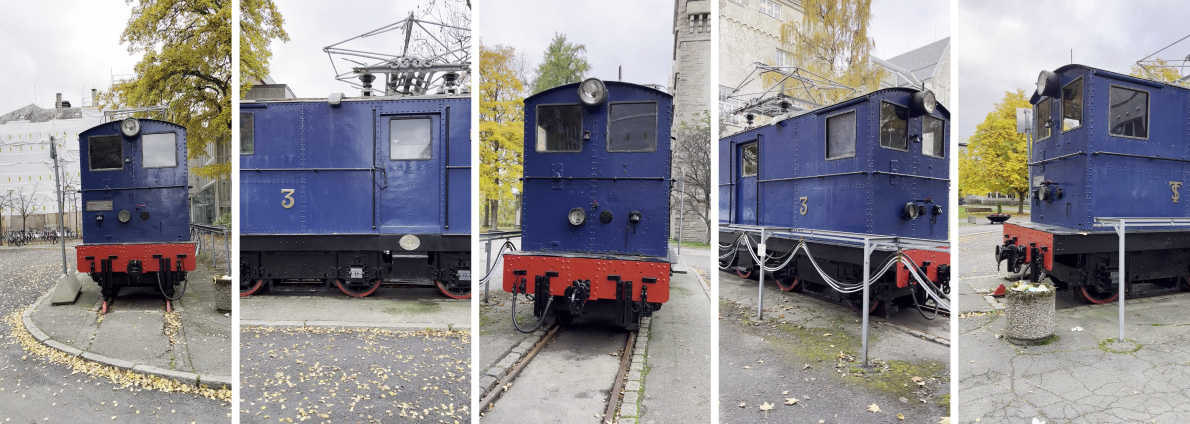
\includegraphics[width=1.0\textwidth]{figures/ohma_electra.png}
    \caption{Unbounded scene: The dataset of Ohma Electra is ~47 seconds long, captured at 30 FPS. The dataset contains 1416 images.}
    \label{fig:ohma-electra}
\end{figure}
\begin{figure}[!h]
    \centering
    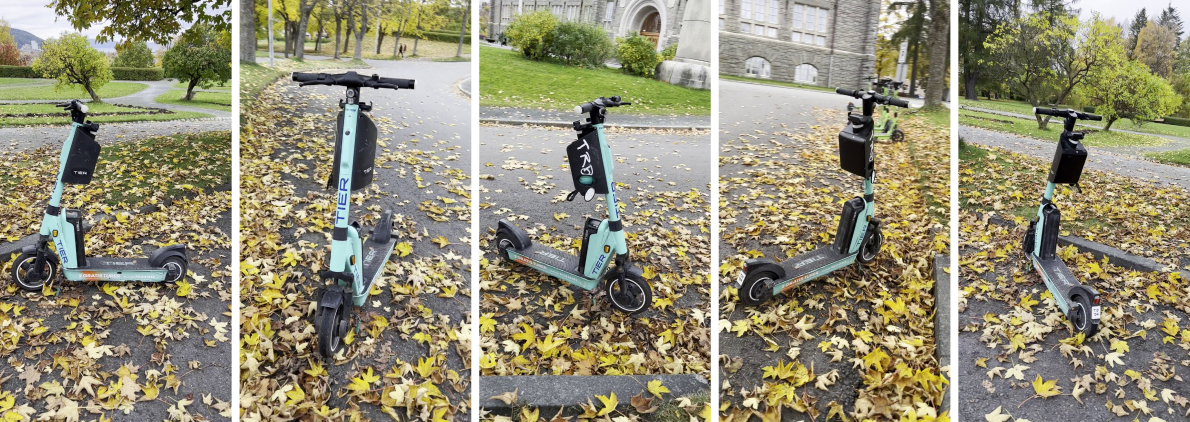
\includegraphics[width=1.0\textwidth]{figures/tier.png}
    \caption{Unbounded scene: The dataset of an electric scooter is ~15 seconds long, captured at 30 FPS. The dataset contains 446 images}
    \label{fig:tier}
\end{figure}

\begin{figure}[!ht]
    \centering
    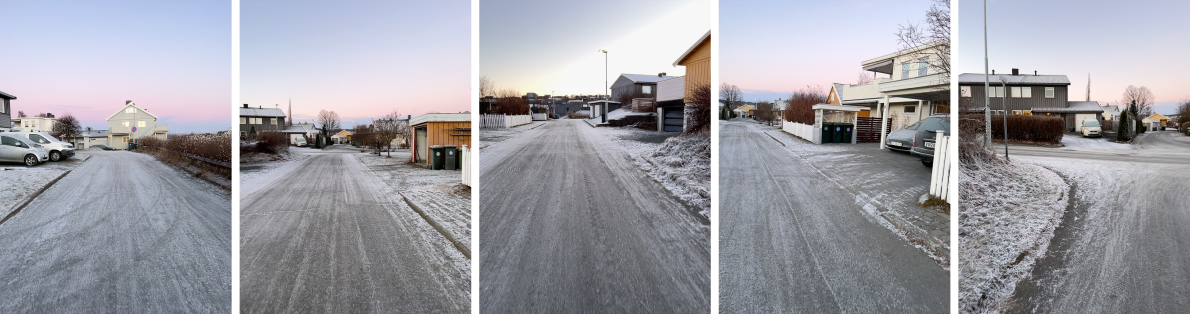
\includegraphics[width=1.0\textwidth]{figures/streetview-dataset.png}
    \caption{Large outdoor, unbounded scene: The dataset of a street in Trondheim is originally caught with the Polycam app. The dataset contains 600 images.}
    \label{fig:streetview-dataset}
\end{figure}
\begin{figure}[h]
    \centering
    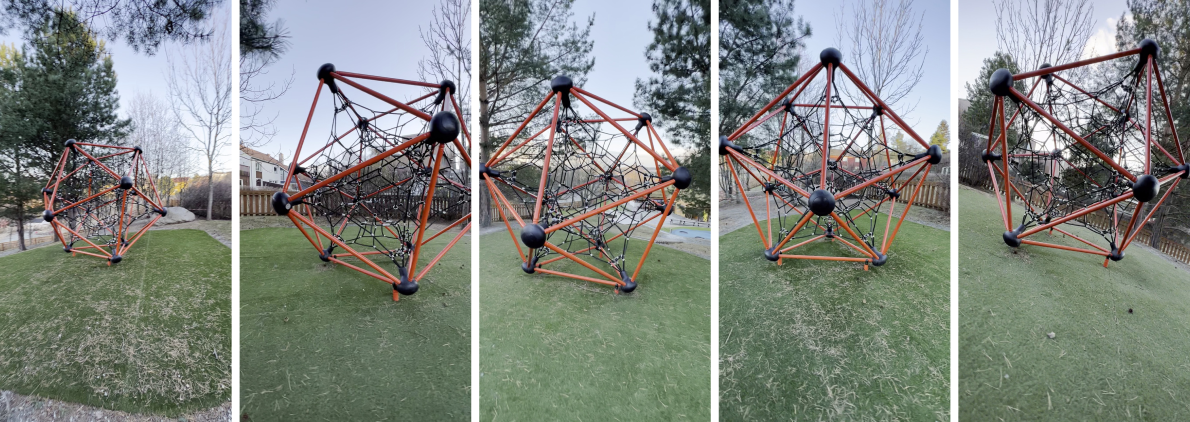
\includegraphics[width=1.0\textwidth]{figures/octahedron-dataset.png}
    \caption{Octahedron dataset. Caught with an iPhone at 0.5x zoom.}
    \label{fig:octahedron-dataset}
\end{figure}
\begin{figure}[h]
    \centering
    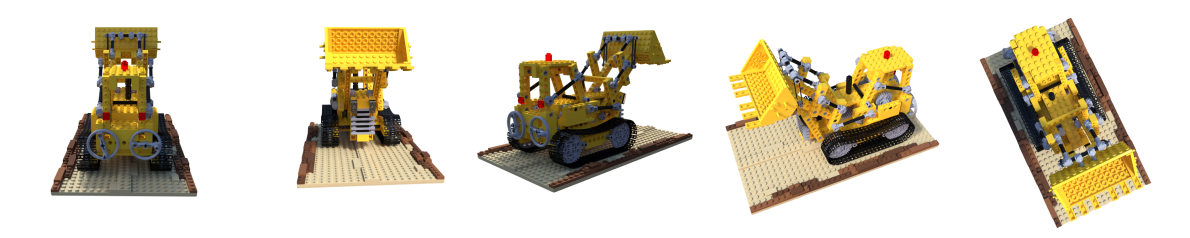
\includegraphics[width=1.0\textwidth]{figures/lego-dataset.png}
    \caption{Blender scene: The dataset of a lego tractor. This dataset is one of the benchmarks in the original NeRF paper. The dataset contains 100 images.}
    \label{fig:lego-dataset}
\end{figure}
\begin{figure}[h]
    \label{fig:fox-dataset}
    \centering
    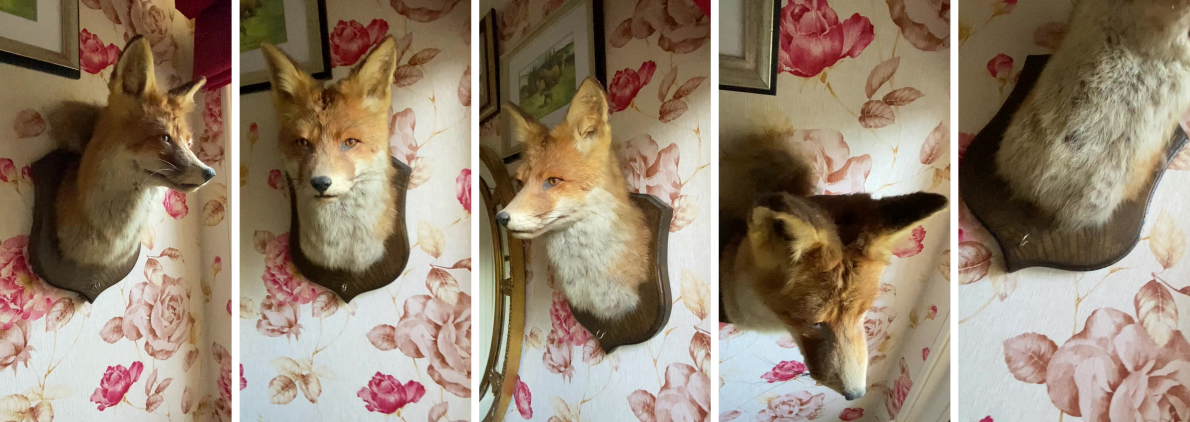
\includegraphics[width=1.0\textwidth]{figures/fox-dataset.png}
    \caption{Bounded scene: The dataset of a stuffed fox on a wall. This dataset is one of the datasets from the instant-ngp repository.}
    \label{fig:my_label}
\end{figure}
\chapter{Results}

\begin{comment}

Experiments:
- Explore the impact of capturing
    - Capturing NeRFs in different ways
        - Walking, standing still, sparsely, densely, linearly, around an object
    - Capturing video, images, polycam
        - Better/worse quality with polycam or COLMAP
    - Capturing different kind of scenes
        - Bounded/Unbounded
    - Capturing in different conditions
    - Capturing 
    
- Explore the impact of dataset size
    - Extract different amounts of images from the video
        - Simulate driving by walking up and back a street multiple times
    - How much data is required until COLMAP becomes a bottleneck

- Explore the impact of area-size
    - Remember to point out that area is poorly defined since scale is perspective relative, depending on the level of detail you want.
    - Area must be defined for a certain scene type. E.g. street view, aerial view, unbounded in multiple directions, bounded in all directions

- Explore the impact of different methods
    - instant-npg, nerfacto, NeRF

Metrics
- Quantitative
    - PSNR, LPIPS, SSIM
- Qualitative
    - Compare images side-by-side



Research questions:
- To what extent does a good capture impact the result of a NeRF
- How much data is required until COLMAP becomes a bottleneck?
- What is the capacity of a NeRF when optimizing a street view scene?

SCENES:
- Bounded scene
- Unbounded scene
- Walking
- Standing still
- Street-view

\end{comment}



\section{Dataset}
\begin{figure}[!h]
    \centering
    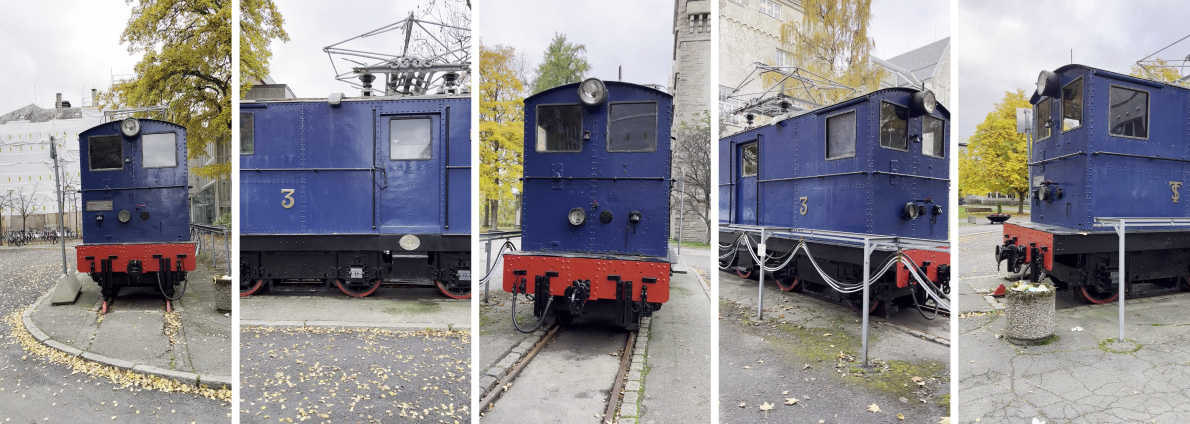
\includegraphics[width=1.0\textwidth]{figures/ohma_electra.png}
    \caption{Unbounded scene: The dataset of Ohma Electra is ~47 seconds long, captured at 30 FPS. The dataset contains 1416 images.}
    \label{fig:ohma-electra}
\end{figure}
\begin{figure}[!h]
    \centering
    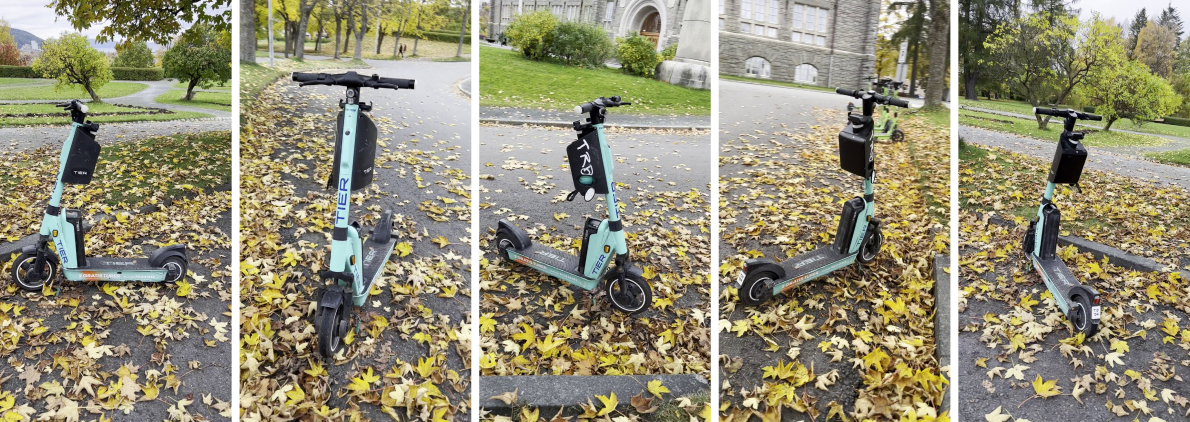
\includegraphics[width=1.0\textwidth]{figures/tier.png}
    \caption{Unbounded scene: The dataset of an electric scooter is ~15 seconds long, captured at 30 FPS. The dataset contains 446 images}
    \label{fig:tier}
\end{figure}




\section{Dataset size}
We explore the impact of sampling different number of images from a video. The input video of Ohma Electra \cite{data:object-unbounded-ohma} is 47 seconds long, captured at 30 FPS resulting in 1410 total frames. Leveraging FFMPEG we sample frames at 4 increasingly dense levels.

\begin{comment}
\begin{table}[h]
\centering
\begin{tabular}{ccccccc}
\hline
\# Samples & PSNR $\uparrow$ & SSIM $\uparrow$ & LPIPS $\downarrow$ & Process Time & Training Time & Evaluate Time \\ \hline
5\%                       & 17.955    & 0.458     & 0.338    & 02:37    & 29:03    & 00:19    \\
10\%                      & 19.422    & 0.505     & 0.280    & 06:10    & 28:31    & 00:24    \\
15\%                      & 19.841    & 0.537     & 0.268    & 12:50    & 28:39    & 00:32    \\
20\%                      & 20.341    & 0.555     & 0.269    & 18:17    & 28:24    & 00:35    \\
25\%                      & 20.118    & 0.548     & 0.263    & 30:05    & 49:08    & 01:15    \\
40\%                      & 22.371    & 0.649     & 0.258    & 58:01    & 28:50    & 01:13    \\
50\%                      & 21.738    & 0.623     & 0.263    & -    & -    & -    \\
75\%                      & -    & -     & -    & -    & -    & -    \\
\multicolumn{1}{l}{100\%} & -    & -     & -    & -    & -    & -    \\ \hline
\end{tabular}
\caption{An overview of how dataset size impacts render-quality and process-, training- and evaluation-time. Trained on \autoref{fig:ohma-electra} with a vanilla Nerfacto pipeline}
\label{tab:colmap-dataset-size}
\end{table}
\end{comment}

\begin{table}[h]
\centering
\begin{tabular}{|l|llllll|}
\hline
\multicolumn{7}{|c|}{\textbf{Ohma Electra scene, \autoref{fig:ohma-electra}}} \\
\hline
\% Frames & PSNR $\uparrow$ & SSIM $\uparrow$ & LPIPS $\downarrow$ & Process & Training & Evaluate \\ \hline
20\%        & 19.692    & 0.523     & 0.272    & 00:36:55    & 20:40    & 00:44    \\
25\%        & 20.043    & 0.544     & 0.269    & 00:57:09    & 19:06    & 00:50    \\
33\%        & 20.135    & 0.547     & 0.273    & 01:22:08    & 20:15    & 01:05    \\
50\%        & 21.103    & 0.590     & 0.273    & 02:47:07    & 20:56    & 01:30    \\
100\%       & -    & -     & -    & -    & -    & -    \\
\hline
\end{tabular}
\caption{An overview of how dataset size impacts render-quality and process-, training- and evaluation-time. Trained on the ohma-electra dataset, as shown in \autoref{fig:ohma-electra}, with a default Nerfacto pipeline}
\label{tab:colmap-dataset-size}
\end{table}

Increasing the dataset size increases the amount of time required to retrieve the camera poses, given they're not known a priori. As discussed in \autoref{sec:colmap}, COLMAP has several different feature matching algorithms, e.g. exhaustive, sequential, and vocabulary tree matching. The choice of a matching algorithm should depend on the type of capture, e.g. if the source of the sampled images is a video it entails that subsequent frames have a certain overlap and makes sequential matching a sensible choice. The time complexity of COLMAP and its matching algorithms is important as the dataset size increases, as it might consume a lot of the time in the overall process-train-render pipeline. An overview of the selected matching algorithms' complexities can be seen in \autoref{tab:colmap-feature-complexity}.

\section{Area size}
We explore the impact of area size. Area in itself is poorly defined in the context of NeRF, since scale is perspective relative, depending on the level of detail you want. A single NeRF can efficiently represent a 3D model of the entire world, but the level of detail won't be satisfactory as you try to render detailed images. In this experiment we'll use a self-captured scene as the benchmark for area-related experiments. The scene \cite{data:streetview} is captured on a relatively straight street, bounded by houses on each side. 

\begin{table}[h] 
\centering
\begin{tabular}{ccccc}
\hline
Metric & 50m & 100m & 200m & 400m \\ \hline
PSNR   & -   & -    & -    & -    \\
LPIPS  & -   & -    & -    & -    \\
SSIM   & -   & -    & -    & -    \\ \hline
\end{tabular}
\label{tab:area-size}
\end{table}

\section{Different methods}
There are multiple different methods proposed for reconstructing 3D scenes and rendering novel views.

\begin{table}[h]
\centering
\begin{tabular}{|lcccc|}
\hline
\multicolumn{5}{|c|}{\textbf{Fox scene, \autoref{fig:fox-dataset}}} \\ 
\hline
Method  & PSNR $\uparrow$ & SSIM $\uparrow$ & LPIPS $\downarrow$& Time  \\ 
\hline
NeRF        & -    & -     & -    & -    \\
mip-NeRF    & -    & -     & -    & -    \\
instant-ngp & 26.370    & 0.863     & 0.214    & 47:45    \\
Nerfacto    & 27.698    & 0.859     & 0.190    & 31:28    \\
\hline

\hline
\multicolumn{5}{|c|}{\textbf{Ohma Electra scene, \autoref{fig:ohma-electra}}} \\ 
\hline
Method  & PSNR $\uparrow$ & SSIM $\uparrow$ & LPIPS $\downarrow$& Time  \\ 
\hline
NeRF        & -    & -     & -    & -    \\
mip-NeRF    & -    & -     & -    & -    \\
instant-ngp & -    & -     & -    & -    \\
Nerfacto    & 20.135    & 0.547     & 0.273    & 20:15    \\ 
\hline

\hline
\multicolumn{5}{|c|}{\textbf{Lego scene, \autoref{fig:ohma-electra}}} \\ 
\hline
Method  & PSNR $\uparrow$ & SSIM $\uparrow$ & LPIPS $\downarrow$& Time  \\ 
\hline
NeRF        & -    & -     & -    & -    \\
mip-NeRF    & -    & -     & -    & -    \\
instant-ngp (Default)     & -    & -     & -    & -    \\
instant-ngp (Adjusted)     & 33.854    & 0.969     & 0.0128    & 21:56    \\
Nerfacto (Default)    & 8.922    & 0.576     & 0.586    & 28:39    \\ 
Nerfacto (Adjusted)    & 19.544    & 0.759     & 0.113    & 28:05    \\ 
\hline
\end{tabular}
\caption{Same scene pre-processed in the same way with the default amount of frames and trained for equal amounts of epochs.}
\label{tab:method-comparison}
\end{table}




\section{Capturing}
\subsection{Polycam vs. COLMAP}



% From Discord thread
\textbf{Wavy artifacts in Nerfacto:}
AFAIK those wavy artifacts are from how the nerfacto model does ray sampling. Sometimes for very thin objects, none of the samples across a ray will land on it, causing it not to be visible in the rendering 

\textbf{Better results with another model?}
One of the reasons nerfacto is so fast is because it learns the distribution of weight across a ray, then samples from that distribution to get the ray samples. This means you aren't sampling where you don't need to, but also you might miss thin structures. Other methods might use more simple ray samplers that would densely sample across the ray, but would end up being a good bit slower to train/render

\chapter{Conclusion}

\begin{comment}
- Loop back to the introduction, review - claim - agenda
    - In this thesis, we have seen how we can reconstruct 3D scenes and render novel views by optimizing NeRFs on 2D input images.
    - The pipeline for creating NeRFs has become greatly simplified recently. As we've seen we can without problems optimize a NeRF in ~4.5 minutes.
\end{comment}

\section{Future work}
Scaling NeRFs to larger scenes isn't trivial. As we've explored, the underlying MLP only has a certain capacity. If we were to increase the capacity training times would increase and rendering times would scale linearly. Rendering is already an expensive operation which further supports the claim for another solution. We've discussed Block-NeRF which decouples rendering times and the ability to reconstruct large scenes by leveraging multiple NeRFs to reconstruct an area.

There aren't a lot of papers exploring large-scale NeRFs. This might be due to the amount of data needed and the corresponding data capture endeavor. In future work, it would be interesting to explore the balance between representing scenes with a single NeRF and when it would make sense to split the scenes into separate NeRFs.

%\chapter{Using the Document Class}
\label{chap:usage}

\section{Thesis Setup and Language Selection}
\label{sec:setup}

The document class is initialized by issuing the \texttt{\textbackslash documentclass[]\{ntnuthesis\}} at the beginning of your \texttt{.tex} file. The thesis language should be given as an option. Currently British English (class option \texttt{[british]}), American English (class option \texttt{[american]}), Norwegian Bokmål (class option \texttt{[norsk]}) and Norwegian Nynorsk (class option \texttt{[nynorsk]}) are supported.\footnote{Disclaimer: this unfortunate naming of the Norwegian language options follows from the naming conventions of the \texttt{babel} package.}

There is also the \texttt{titlepage} class option that triggers the generation of a simple title page that can be used as a placeholder when writing the thesis. This option should be removed before handing in the thesis. Instead the official NTNU titlepage for the corresponding thesis type should be added as described on Innsida.\footnote{see \url{https://innsida.ntnu.no/wiki/-/wiki/English/Finalizing+the+bachelor+and+master+thesis} for bachelor and master, and \url{https://innsida.ntnu.no/wiki/-/wiki/English/Printing+your+thesis} for PhD.}

\section{Title, Author, and Date}

In the preample of the \texttt{.tex} file, the thesis title should be set with the \texttt{\textbackslash title\{\}} command. The title will appear on the titlepage as well as in the running header of the even numbered pages. If the title is too long for the header, you can use \texttt{\textbackslash shorttitle\{\}} to set a version for the header.

The authors should be listed with full names in the \texttt{\textbackslash author\{\}} command. If there are several authors, they should be separated with \texttt{\textbackslash and}, e.g., like this: \texttt{\textbackslash author\{Anne Andersen \textbackslash and Bjørn Bjørnsen\}}. For the running headers, you may want to use \texttt{\textbackslash shortauthor}, e.g. like this: \texttt{\textbackslash shortauthor\{A. Andersen and B. Bjørnsen\}} or even \texttt{\textbackslash shortauthor\{Andersen et al.\}}.

Use \texttt{\textbackslash date\{\}} to set the date of the document. It will only  appear on the temporary title page. To keep track of temporary versions, it can be a good idea to use \texttt{\textbackslash date\{\textbackslash today\}} while working on the thesis. You may also add copyright and licence information in this field.

\section{Page Layout}

The document class is designed to work with twosided printing. This means that all chapters start on odd (right hand) pages, and that blank pages are inserted where needed to make sure this happens. However, since the theses are very often read on displays, the margins are kept the same on even and odd pages in order to avoid that the page is jumping back and forth upon reading.

To avoid blank pages when rendering the thesis, you can enable the \texttt{oneside} option in the \texttt{thesis.tex} file. Just add 'oneside' to the document class options on the first line, and recompile.

\section{Structuring Elements}

The standard \LaTeX{} elements for document structure are supported: chapter, section, and:

\subsection{This is a \texttt{\textbackslash subsection\{\}}}

Short subsection text here.

\subsubsection{This is a \texttt{\textbackslash subsubsection\{\}}}

Short subsubsection text here.

\paragraph{This is a \texttt{\textbackslash paragraph\{\}}}

Short paragraph text here.

Chapters, sections, and subsections will be included in the table of contents, whereas the lower level structuring elements will not appear there. Don't use too many levels of headings; how many are appropriate, will depend on the size of the document. Also, don't use headings too frequently.

Make sure that the chapter and section headings are correctly capitalised depending on the language of the thesis, e.g., `\emph{Correct Capitalisation of Titles in English}' vs. `\emph{Korrekt staving av titler på norsk}'.

Simple paragraphs are the lowest structuring elements and should be used the most. They are made by leaving one (or more) blank line(s) in the \texttt{.tex} file. In the typeset document they will appear indented and with no vertical space between them.

\section{Lists}

Numbered and unnumbered lists, i.e., the \texttt{enumerate} and \texttt{itemize} environments, are used just as in regular \LaTeX{}, but are typeset somewhat more densely and with other labels. Unnumbered list:
\begin{itemize}
    \item first item
    \item second item
    \begin{itemize}
        \item first subitem
        \item second subitem
        \begin{itemize}
            \item first subsubitem
            \item second subsubitem
        \end{itemize}
    \end{itemize}
    \item last item
\end{itemize}
Numbered list:
\begin{enumerate}
    \item first item
    \item second item
    \begin{enumerate}
        \item first subitem
        \item second subitem
        \begin{enumerate}
            \item first subsubitem
            \item second subsubitem
        \end{enumerate}
    \end{enumerate}
    \item last item
\end{enumerate}

For description lists, see usage in, e.g., \cref{sec:frontmatter}.

\section{Figures}

Figures are placed in the \texttt{figure} environment. An example is shown in \cref{fig:mapNTNU}. Figures are floats, hence they will float freely around in the document in accordance with standard \LaTeX{} behaviour. You may want to try to override \LaTeX{}'s default placement by using the \texttt{h} (here), \texttt{t} (top of page), \texttt{b} (bottom of page), and \texttt{p} (separate page) options in order of priority. If you provide an alternate (typically shorter) caption in square brackets, it will be used in the list of figures. Use \texttt{\textbackslash includegraphics[]\{\}} with options \texttt{scale} or \texttt{width} to include the graphics file. The caption should be placed \emph{below} the figure. If the caption consists of a single sentence fragment (incomplete sentence), it should not be punctuated. Given the shape and size of the figure, the figure caption can appear too close or too far from the figure. To deal with this, vertical space, either positive or negative, can be added before and/or after the caption command using the \texttt{\textbackslash vspace{}} command.

\begin{figure}[htbp]  % order of priority: h here, t top, b bottom, p page
  \centering
  \includegraphics[width=.5\textwidth]{figures/kart_student}
  \caption[Map of NTNU Campuses]{The map shows the three main campuses of NTNU.}
  \label{fig:mapNTNU}
\end{figure}

For figures compsed of several sub-figures, the \texttt{caption} and \texttt{subcaption} packages have been preloaded. See \cref{fig:subfig} with \cref{sfig:a,sfig:b} for an example. For more details on alignment etc., see the Overleaf documentation.\footnote{\url{https://www.overleaf.com/learn/latex/How_to_Write_a_Thesis_in_LaTeX_(Part_3):_Figures,_Subfigures_and_Tables}}

\begin{figure}
    \centering
    \begin{subfigure}[b]{.45\textwidth}
        \centering
        \includegraphics[width=\textwidth]{figures/kart_student.png}
        \caption{First sub-figure}
        \label{sfig:a}
    \end{subfigure}
    \hfill
    \begin{subfigure}[b]{.45\textwidth}
        \centering
        \includegraphics[width=\textwidth]{figures/kart_student.png}
        \caption{Second sub-figure}
        \label{sfig:b}
    \end{subfigure}
    \caption{A figure composed of two sub-figures. It has a long caption in order to demonstrate how that is typeset.}
    \label{fig:subfig}
\end{figure}

You can make nice graphs directly from data files using \texttt{gnuplot}, but it is expensive on every compilation.  The code is included in the
raw latex as a comment so you can uncomment that code to see how it works.
% , for an example, see \cref{fig:examplegnuplot}.
%
%\begin{figure}[htbp]
%  \centering
%    \begin{gnuplot}[terminal=epslatex,terminaloptions={size 8cm,6cm color}]
%        set xlabel "age"
%        set ylabel "IQ"
%        set key autotitle columnhead
%        set title "age vs IQ"
%        set yrange [0:160]
%        set datafile separator ","
%        plot "csvtables/ageiq.csv" using 1:2 with boxes
%    \end{gnuplot}
%  \caption[An example of Integrated Graph]{This is a gnuplot graph read from a file. Also this figure has a long caption in order to demonstrate how that is typeset.}
%  \label{fig:examplegnuplot}
%\end{figure}

\section{Tables}

Tables are placed in the \texttt{table} environment. An example is given in \cref{tab:example1}. Like figures, tables float freely around in the document in accordance with standard \LaTeX{} behaviour. The table caption should be placed \emph{above} the table. If the caption consists of a single sentence fragment (incomplete sentence), it should not be punctuated.

\begin{table}
  \centering
  \caption{A simple, manually formatted example table}
  \label{tab:example1}
  \begin{tabular}{cc}
    \hline
    age  & IQ \\
    \hline
    10   & 110 \\
    20   & 120 \\
    30   & 145 \\
    40   & 120 \\
    50   & 100 \\
    \hline
  \end{tabular}
\end{table}

Tables can also be automatically generated from CSV files using the \texttt{simplecsv} and \texttt{booktab} packages. See \cref{tab:examplecsv} for an example.

\begin{table}[tbp]
  \centering
  \caption[A simple example table generated from a CSV file]{A simple example table generated from a CSV file using \texttt{simplecsv} and \texttt{booktab}}
  \label{tab:examplecsv}
  \csvautobooktabular{csvtables/ageiq.csv}
\end{table}

\section{Listings}

Code listings are included by means of the \texttt{listings} package. Code examples can be read from file or provided inline, and should be given a caption for cross referencing and for appearance in the list of code listings in the thesis frontmatter. If all your code examples are written in the same programming language, you can use, e.g., \texttt{\textbackslash lstset\{language=Python\}} to set the language once and for all. The code is set with the monospace font, and the font size is reduced to allow for code lines up to at least 80 characters without causing line breaks. Options for programming languages, line numbering etc. are provided. Unlike figures and tables, code listings are not floating objects, and will appear at the same position in the typeset document as in the \texttt{.tex} file. If the caption consists of a single sentence fragment (incomplete sentence), it should not be punctuated.

\lstinputlisting[
    caption={Python example from file},
    label=lst:pythonfile,
    language=Python
]{listings/example.py}

\lstinputlisting[%
    caption={C++ example from file},
    label=lst:cppfile,
    language=C++,
    numbers=left
]{listings/example.cc}

\begin{lstlisting}[
    caption={Python code in \LaTeX{} document},
    label=lst:pythondoc,
    language=Python]
import numpy as np
import matplotlib.pyplot as plt

x = np.linspace(0, 1)
y = np.sin(2 * np.pi * x)

plt.plot(x, y)
plt.show()
\end{lstlisting}

\begin{lstlisting}[
    caption={C++ code in \LaTeX{} document},
    label=lst:cppdoc,
    language=C++]
#include <iostream>
using namespace std;

int main()
{
  cout << "Hello, World!" << endl;
  return 0;
}
\end{lstlisting}

\section{Equations}

Equations are typeset as normally in \LaTeX{}. It is common to consider equations part of the surrounding sentences, and include punctuation in the equations accordingly, e.g.,
\begin{equation}
    f(x) = \int_1^x \frac{1}{y}\,dy = \ln x\,.
    \label{eq:logarithm}
\end{equation}
For more advanced symbols like, e.g., $\mathbb{R}, \mathbb{Q}$, the \texttt{amssymb} package is preloaded, and for more advanced mathematical layout the \texttt{amsmath} behaviour is obtained through the \texttt{mathdesign} package. Confer the overleaf documentation for details.\footnote{\url{https://www.overleaf.com/learn/latex/Mathematical_expressions}}

\section{Fonts}

Bitstream Charter at 11pt with the corresponding Mathdesign math fonts have been selected as the main fonts for the thesis template. For code examples, the monospaced font should be used – for this, a scaled version of the DejaVuSansMono to match the main font is preselected. If you would like to use an accompanying sans serif font, the BeraSans has been made available. The standard \LaTeX{} font commands should be used to switch between fonts, e.g.,
\texttt{\textbackslash textit\{\}} \textit{for italics},
\texttt{\textbackslash textbf\{\}} \textbf{for bold face},
\texttt{\textbackslash texttt\{\}} \texttt{for mono spaced}, and
\texttt{\textbackslash textsf\{\}} \textsf{for sans serif}.
For generic \emph{emphasis}, \texttt{\textbackslash emph\{\}} should be applied.

\section{Cross References}
\label{sec:crossref}

For cross references, i.e., references within the document, the \texttt{\textbackslash cref\{\}} command provided byt the \texttt{cleveref} package should be used. Labels are inserted in the document in the standard \LaTeX{} manner. They are case sensitive, so, e.g., a label immediately after a section command refers to that section, while a label within, e.g., a table environment refers to the table. The \texttt{\textbackslash cref\{\}} command also generates the corresponding text. If the document is in English (class options \texttt{british} or \texttt{american}), the cross references are capitalised, whereas if it is in Norwegian (class options \texttt{norsk} or \texttt{nynorsk}), they are not. If you are writing in Norwegian, you should use \texttt{\textbackslash Cref\{\}} at the beginning of a sentence to ensure that the cross reference is correctly capitalised. For examples on usage, see \cref{sec:crossref} in \cref{chap:usage}, \cref{tab:example1}, \cref{fig:mapNTNU}, \cref{eq:logarithm}, \cref{lst:cppfile}, \cref{paper:scrutiny}, and \cref{app:additional}. \Cref{app:additional} at the beginning of a sentence.

The cross references are made into active hyperlinks in the resulting PDF document by the use of the \texttt{hyperref} package. The colour of the links is set to black for best appearance on print. This can easily be changed by the author by the use of the \texttt{\textbackslash hypersetup\{\}} command.

\section{Glossary and Acronyms}
The template comes with the ability to create a glossary and acronym list. To add entries to one of these lists, add them to the \texttt{glossary.tex} file.
All uses of the acronym and glossary functions will create a clickable link that references the corresponding entry in one of the lists. All entries in the lists will also contain page references to all places it has been used.
\subsection{Using Acronyms}
To render acronyms, you have three options:
\begin{itemize}
  \item \texttt{\textbackslash acrlong\{ \}} prints the phrase the acronym stands for, e.g. \texttt{\textbackslash acrlong\{gcd\}} displays \acrlong{gcd}.
  \item \texttt{\textbackslash acrshort\{ \}} prints the acronym, e.g. \texttt{\textbackslash acrshort\{gcd\}} displays \acrshort{gcd}.
  \item \texttt{\textbackslash acrfull\{ \}} prints both the acronym and its definition, e.g. \texttt{\textbackslash acrfull\{gcd\}} displays \acrfull{gcd}.
\end{itemize}

\subsection{Using Glossary}
\begin{itemize}
  \item \texttt{\textbackslash gls\{ \}} prints the term in lowercase, e.g. \texttt{\textbackslash gls\{maths\}} displays \gls{maths}.
  \item \texttt{\textbackslash Gls\{ \}} prints the term in with first letter in uppercase, e.g. \texttt{\textbackslash Gls\{maths\}} displays \Gls{maths}.
  \item \texttt{\textbackslash glspl\{ \}} prints the term in plural form, e.g. \texttt{\textbackslash glspl\{bibliography\}} displays \glspl{bibliography}.
  \item \texttt{\textbackslash Glspl\{ \}} prints the term in plural form capitalized, e.g. \texttt{\textbackslash Glspl\{bibliography\}} displays \Glspl{bibliography}.
\end{itemize}


\section{Bibliography}

The \gls{bibliography} is typset using the \texttt{biblatex} package with the \texttt{biber} backend. The default citation style is \texttt{numeric-comp}, and the default bibliography style is \texttt{numeric}. This produces a bibliography similar to, but not completely according to, the so-called Vancouver style. With this setup, a single \texttt{\textbackslash cite\{\}} command will give a number only~\cite{landes1951scrutiny}, and \texttt{\textbackslash textcite\{\}} will give author and number like this: \textcite{landes1951scrutiny}. If you would like to give the full reference of a paper within the thesis, e.g., in a list of included papers, use \texttt{\textbackslash fullcite\{\}} like this: \fullcite{landes1951scrutiny}.

\section{Included Papers}

If you are writing a compiled PhD thesis (and probably only then – see \cref{sec:compiledphd}), you will need to attach the papers containing the main contribution of the thesis. This can be done issuing the \texttt{paper} environment. It takes two arguments: (i) the PDF file, and (ii) a label for cross referencing. See \cref{paper:scrutiny} for an example.

\section{Appendices}

Additional material that does not fit in the main thesis but may still be relevant to share, e.g., raw data from experiments and surveys, code listings, additional plots, pre-project reports, project agreements, contracts, logs etc., can be put in appendices. Simply issue the command \texttt{\textbackslash appendix} in the main \texttt{.tex} file, and then the following chapters made by \texttt{\textbackslash chapter\{\}} become appendices. See \cref{app:additional} for an example.

%\chapter{Thesis Structure}

The structure of the thesis, i.e., which chapters and other document elements that should be included, depends on several factors such as the study level (bachelor, master, PhD), the type of project it describes (development, research, investigation, consulting), and the diversity (narrow, broad). Thus, there are no exact rules for how to do it, so whatever follows should be taken as guidelines only.

A thesis, like any book or report, can typically be divided into three parts: front matter, body matter, and back matter. Of these, the body matter is by far the most important one, and also the one that varies the most between thesis types.

\section{Front Matter}
\label{sec:frontmatter}

The front matter is everything that comes before the main part of the thesis. It is common to use roman page numbers for this part to indicate this. The minimum required front matter consists of a title page, abstract(s), and a table of contents. A more complete front matter, in a typical order, is as follows.

\begin{description}
    \item[Title page:] The title page should, at minimum, include the thesis title, authors and a date. A more complete title page would also include the name of the study programme, and possibly the thesis supervisor(s). See \cref{sec:setup}.
    \item[Abstracts:] The abstract should be an extremely condensed version of the thesis. Think one sentence with the main message from each of the chapters of the body matter as a starting point. \textcite{landes1951scrutiny} have given some very nice instructions on how to write a good abstract. A thesis from a Norwegian Univeristy should contain abstracts in both Norwegian and English irrespectively of the thesis language (typically with the thesis language coming first).
    \item[Dedication:] If you wish to dedicate the thesis to someone (increasingly common with increasing study level), you may add a separate page with a dedication here. Since a dedication is a personal statement, no template is given. Design it according to your preference.
    \item[Acknowledgements:] If there is someone who deserves a `thank you', you may add acknowledgements here. If so, make it an unnumbered chapter, i.e., \texttt{\textbackslash chapter*\{Acknowledgements\}}.
    \item[Table of contents:] A table of contents should always be present in a document at the size of a thesis. It is generated automatically using the \texttt{\textbackslash tableofcontents} command. The one generated by this document class also contains the front matter and unnumbered chapters.
    \item[List of figures:] If the thesis contains many figures that the reader might want to refer back to, a list of figures can be included here. It is generated using \texttt{\textbackslash listoffigures}.
    \item[List of tables:] If the thesis contains many tables that the reader might want to refer back to, a list of tables can be included here. It is generated using \texttt{\textbackslash listoftables}.
    \item[List of code listings:] If the thesis contains many code listings that the reader might want to refer back to, a list of code listings can be included here. It is generated using \texttt{\textbackslash lstlistoflistings}.
    \item[Other lists:] If there are other list you would like to include, this would be a good place. Examples could be lists of definitions, theorems, nomenclature, abbreviations, glossary etc. There are no standards for this, but many lists can be generated using the \texttt{description} environment (like, e.g., this list of possible front matter content) within a separate \texttt{\textbackslash chapter*\{\}}.
    \item[Preface or Foreword:] A preface or foreword is a good place to make other personal statements that do not fit whithin the body matter. This could be information about the circumstances of the thesis, your motivation for choosing it, or possibly information about an employer or an external company for which it has been written. Again, use, e.g., \texttt{\textbackslash chapter*\{Preface\}}.
\end{description}

\section{Body Matter}

The body matter consists of the main chapters of the thesis. It starts the Arabic page numbering with page~1. There is a great diversity in the structure chosen for different thesis types. Common to almost all is that the first chapter is an introduction, and that the last one is a conclusion followed by the bibliography.

\subsection{Development Project}
\label{sec:development}

For many bachelor and some master projects in computer science, the main task is to develop something, typically a software prototype, for an `employer' (e.g., an external company or a research group). A thesis describing such a project is typically structured as a software development report whith more or less the following chapters:

\begin{description}
    \item[Introduction:] The introduction of the thesis should take the reader all the way from the big picture and context of the project to the concrete task that has been solved in the thesis. A nice skeleton for a good introduction was given by \textcite{claerbout1991scrutiny}: \emph{review–claim–agenda}. In the review part, the background of the project is covered. This leads up to your claim, which is typically that some entity (software, device) or knowledge (research questions) is missing and sorely needed. The agenda part briefly summarises how your thesis contributes.
    \item[Requirements:] The requirements chapter should lead up to a concrete description of both the functional and non-functional requirements for whatever is to be developed at both a high level (use cases) and lower levels (low level use cases, requirements). If a classical waterfall development process is followed, this chapter is the product of the requirement phase. If a more agile model like, e.g., SCRUM is followed, the requirements will appear through the project as, e.g., the user stories developed in the sprint planning meetings.
    \item[Technical design:] The technical design chapter describes the big picture of the chosen solution. For a software development project, this would typically contain the system arcitechture (client-server, cloud, databases, networking, services etc.); both how it was solved, and, more importantly, why this architecture was chosen.
    \item[Development Process:] In this chapter, you should describe the process that was followed. It should cover the process model, why it was chosen, and how it was implemented, including tools for project management, documentation etc. Depending on how you write the other chapters, there may be good reasons to place this chapters somewhere else in the thesis.
    \item[Implementation:] Here you should describe the more technical details of the solution. Which tools were used (programming languages, libraries, IDEs, APIs, frameworks, etc.). It is a good idea to give some code examples. If class diagrams, database models etc. were not presented in the technical design chapter, they can be included here.
    \item[Deployment:] This chapter should describe how your solution can be deployed on the employer's system. It should include technical details on how to set it up, as well as discussions on choices made concerning scalability, maintenance, etc.
    \item[Testing and user feedback:] This chapter should describe how the system was tested during and after development. This would cover everything from unit testing to user testing; black-box vs. white-box; how it was done, what was learned from the testing, and what impact it had on the product and process.
    \item[Discussion:] Here you should discuss all aspect of your thesis and project. How did the process work? Which choices did you make, and what did you learn from it? What were the pros and cons? What would you have done differently if you were to undertake the same project over again, both in terms of process and product? What are the societal consequences of your work?
    \item[Conclusion:] The conclusion chapter is usually quite short – a paragraph or two – mainly summarising what was achieved in the project. It should answer the \emph{claim} part of the introduction. It should also say something about what comes next (`future work').
    \item[Bibliography:] The bibliography should be a list of quality-assured peer-reviewed published material that you have used throughout the work with your thesis. All items in the bibliography should be referenced in the text. The references should be correctly formatted depending on their type (book, journal article, conference publication, thesis etc.). If \texttt{biblatex} is correctly used as proposed by this template, the formatting will be taken care of automatically. The bibliography should not contain links to arbitrary dynamic web pages where the content is subject to change at any point of time. Such links, if necessary, should rather be included as footnotes throughout the document. The main point of the bibliography is to back up your claims with quality-assured material that future readers will actually be able to retrieve years ahead.
\end{description}

\subsection{Research Project}
\label{sec:resesarch}

For many master and some bachelor projects in computer science, the main task is to gain knew knowledge about something. A thesis describing such a project is typically structed as an extended form of a scientific paper, following the so-called IMRaD (Introduction, Method, Results, and Discussion) model:

\begin{description}
    \item[Introduction:] See \cref{sec:development}.
    \item[Background:] Research projects should always be based on previous research on the same and/or related topics. This should be described as a background to the thesis with adequate bibliographical references. If the material needed is too voluminous to fit nicely in the review part of the introduction, it can be presented in a separate background chapter.
    \item[Method:] The method chapter should describe in detail which activities you undertake to answer the research questions presented in the introduction, and why they were chosen. This includes detailed descriptions of experiments, surveys, computations, data analysis, statistical tests etc.
    \item[Results:] The results chapter should simply present the results of applying the methods presented in the method chapter without further ado. This chapter will typically contain many graphs, tables, etc. Sometimes it is natural to discuss the results as they are presented, combining them into a `Results and Discussion' chapter, but more often they are kept separate.
    \item[Discussion:] See \cref{sec:development}.
    \item[Conclusion:] See \cref{sec:development}.
    \item[Bibliography:] See \cref{sec:development}.
\end{description}

\subsection{Monograph PhD Thesis}
\label{sec:monograph}

Traditionally, it has been common to structure a PhD thesis as a single book – a \emph{monograph}. If the thesis is in the form of one single coherent research project, it can be structured along the lines of \cref{sec:resesarch}. However, for such a big work that a PhD thesis constitutes, the tasks undertaken are often more diverse, and thus more naturally split into several smaller research projects as follows:

\begin{description}
    \item[Introduction:] The introduction would serve the same purpose as for a smaller research project described in \cref{sec:development}, but would normally be somewhat more extensive. The \emph{agenda} part should inform the reader about the structure of the rest of the document, since this may vary significantly between theses.
    \item[Background:] Where as background chapters are not necessarily needed in smaller works, they are almost always need in PhD thesis. They may even be split into several chapters if there are significantly different topics to cover. See \cref{sec:resesarch}.
    \item[Main chapters:] Each main chapter can be structured more or less like a scientific paper. Depending on how much is contained in the introduction and background sections, the individual introduction and background sections can be significantly reduced or even omitted completely.
    \begin{itemize}
        \item (Introduction)
        \item (Background)
        \item Method
        \item Results
        \item Discussion
        \item Conclusion
    \end{itemize}
    \item[Discussion:] In addition to the discussions within each of the individual chapters, the contribution of the thesis \emph{as a whole} should be thoroughly discussed here.
    \item[Conclusion:] In addition to the conclusions of each of the individual chapters, the overall conclusion of the thesis, and how the different parts contribute to it, should be presented here. The conclusion should answer to the research questions set out in the main introduction. See also \cref{sec:development}.
    \item[Bibliography:] See \cref{sec:development}.
\end{description}

\subsection{Compiled PhD Thesis}
\label{sec:compiledphd}

Instead of writing up the PhD thesis as a monograph, compiled PhD theses (also known as stapler theses, sandwich theses, integrated theses, PhD by published work) consisting of reproductions of already published research papers are becoming increasingly common. At least some of the papers should already have been accepted for publication at the time of submission of the thesis, and thus have been through a real quality control by peer review.

\begin{description}
    \item[Introduction:] See \cref{sec:monograph}.
    \item[Background:] See \cref{sec:monograph}.
    \item[Main contributions:] This chapter should sum up \emph{and integrate} the contribution of the thesis as a whole. It should not merely be a listing of the abstracts of the individual papers – they are already available in the attached papers, and, as such, not needed here.
    \item[Discussion:] See \cref{sec:monograph}.
    \item[Conclusion:] See \cref{sec:monograph}.
    \item[Bibliography:] See \cref{sec:development}.
    \item[Paper I:] First included paper with main contributions. It can be included verbatim as a PDF. The publishers PDF should be used if the copyright permits it. This should be checked with the SHERPA/RoMEO database\footnote{\url{http://sherpa.ac.uk/romeo/index.php}} or with the publisher. Even when it is no general permission by the publisher, you may write and ask for one.
    \item[Paper II:] etc.
\end{description}

\section{Back Matter}

Material that does not fit elsewhere, but that you would still like to share with the readers, can be put in appendices. See \cref{app:additional}.





\chapter*{\bibname}
\printbibliography[heading=none]

%\input{chapters/papers.tex}

\appendix
%\chapter{Additional Material} \label{app:additional}

\section{Parameters for the training in Nerfstudio}

\subsection{Nerfacto}
\begin{table}[h]
    \begin{tabular}{|l|l|}
    \hline
    Description                                             & Default Value \\
    \hline
    How far along the ray to start sampling.                & 0.05 \\
    How far along the ray to stop sampling.                 & 1000.0 \\
    %Whether to randomize the background color.              & \"last\_sample\" \\
    %Number of samples per ray for the proposal network.     & \(256, 96\) \\
    Number of samples per ray for the nerf network.         & 48 \\
    Sample every n steps after the warmup                   & 5 \\
    Scales n from 1 to proposal\_update\_every over this many steps & 5000 \\
    Number of proposal network iterations.                  & 2 \\
    Use the same proposal network. Otherwise use different ones. & False \\
    Proposal loss multiplier.                               & 1.0 \\
    Distortion loss multiplier.                             & 0.002 \\
    Orientation loss multipier on computed noramls.         & 0.0001 \\
    Predicted normal loss multiplier.                       & 0.001 \\
    Whether to use proposal weight annealing.               & True \\
    Whether to use average appearance embedding or zeros for inference. & True \\
    Slope of the annealing function for the proposal weights & 10.0 \\
    Max num iterations for the annealing function.          & 1000 \\
    Whether use single jitter or not for the proposal networks. & True \\
    Whether to predict normals or not.                      & False \\
    \hline
    \hline
    Description of corresponding proposal density fields    & Default Value \\
    \hline
    Dimension of hidden layer           & 16 \\
    Hashmap size                        & $2^{17}$ \\
    Number of levels of the hashmap     & 5 \\
    Maximum resolution of the hashmap (density field 1)         & 64 \\
    Maximum resolution of the hashmap (density field 2)         & 256 \\
    \hline
    \end{tabular}
    \caption{An overview of the parameters in the default Nerfacto model}
    \label{tab:nerfacto-parameter-overview}
\end{table}

\subsection{Instant-ngp}
\begin{table}[h]
    \centering
    \begin{tabular}{|l|l|}
    \hline
    \textbf{Description} & \textbf{Value} \\ 
    \hline
    Whether to create a scene collider to filter rays. & False \\
    Number of samples in field evaluation. & 24 \\
    Resolution of the grid used for the field. & 128 \\
    Contraction type. & Unbounded Sphere \\
    Cone angle & 0.004 \\
    Minimum step size for rendering. & 0.01 \\
    How far along ray to start sampling. & 0.05 \\
    How far along ray to stop sampling. & 1e3 \\
    Whether to use an appearance embedding. & False \\
    Whether to randomize the background color. & True \\ \hline
    \end{tabular}
    \caption{An overview of the parameters in the default Instant-ngp model}
    \label{tab:instant-ngp-parameter-overview}
\end{table}

\subsection{NeRF}
\begin{table}[h]
    \centering
    \begin{tabular}{|l|l|}
    \hline
    \textbf{Description} & \textbf{Value} \\ 
    \hline
    Number of samples in coarse field evaluation & 64 \\
    Number of samples in fine field evaluation & 128 \\
    Specifies whether or not to include ray warping based on time. & False \\
    \hline
    \end{tabular}
    \caption{An overview of the parameters in the default NeRF model}
    \label{tab:instant-ngp-parameter-overview}
\end{table}

\subsection{mip-NeRF}
\begin{table}[h]
    \centering
    \begin{tabular}{|l|l|}
    \hline
    \textbf{Description} & \textbf{Value} \\ 
    \hline
    Whether to create a scene collider to filter rays.  & True \\
    Near plane collider-plane.                          & 2.0 \\
    Far plane collider-plane.                           & 6.0 \\
    The loss coeficcient for the coarse MLP.            & 1.0 \\
    The loss coeficcient for the fine MLP.              & 1.0 \\
    Number of rays per chunk during eval                & 4096 \\
    \hline
    \end{tabular}
    \caption{An overview of the parameters in the default NeRF model}
    \label{tab:instant-ngp-parameter-overview}
\end{table}


\begin{comment}
    
Additional material that does not fit in the main thesis but may still be relevant to share, e.g., raw data from experiments and surveys, code listings, additional plots, pre-project reports, project agreements, contracts, logs etc., can be put in appendices. Simply issue the command \texttt{\textbackslash appendix} in the main \texttt{.tex} file, and make one chapter per appendix.

If the appendix is in the form of a ready-made PDF file, it should be supported by a small descriptive text, and included using the \texttt{pdfpages} package. To illustrate how it works, a standard project agreement (for the IE faculty at NTNU in Gjøvik) is attached here. You would probably want the included PDF file to begin on an odd (right hand) page, which is achieved by using the \texttt{\textbackslash cleardoublepage} command immediately before the \texttt{\textbackslash includepdf[]\{\}} command. Use the option \texttt{[pages=-]} to include all pages of the PDF document, or, e.g., \texttt{[pages=2-4]} to include only the given page range.

\cleardoublepage
\includepdf[pages=-]{appendices/NTNUProsjektavtale.pdf}
\end{comment}

\end{document}
